


\section{Simulations and Results} \label{sec:Simulation Results}



\subsection{Orbital Crossings} \label{subsec:Orbital Crossings}



        
    


    Following the process laid out in \cref{subsec: computationOfPlanarResonantOrbits} to compute the crossings of planar resonant orbits, code employing the use of pydylan (a Python interface to the Dynamically Leveraged Automated (N) Multibody Trajectory Optimization software, \cite{beeson2022dynamically}) was written to plot these crossings within the accessible region for several different orbital families.


    \begin{figure}[ht] \label{fig:orbital crossings plotted}
    	\centering
        % 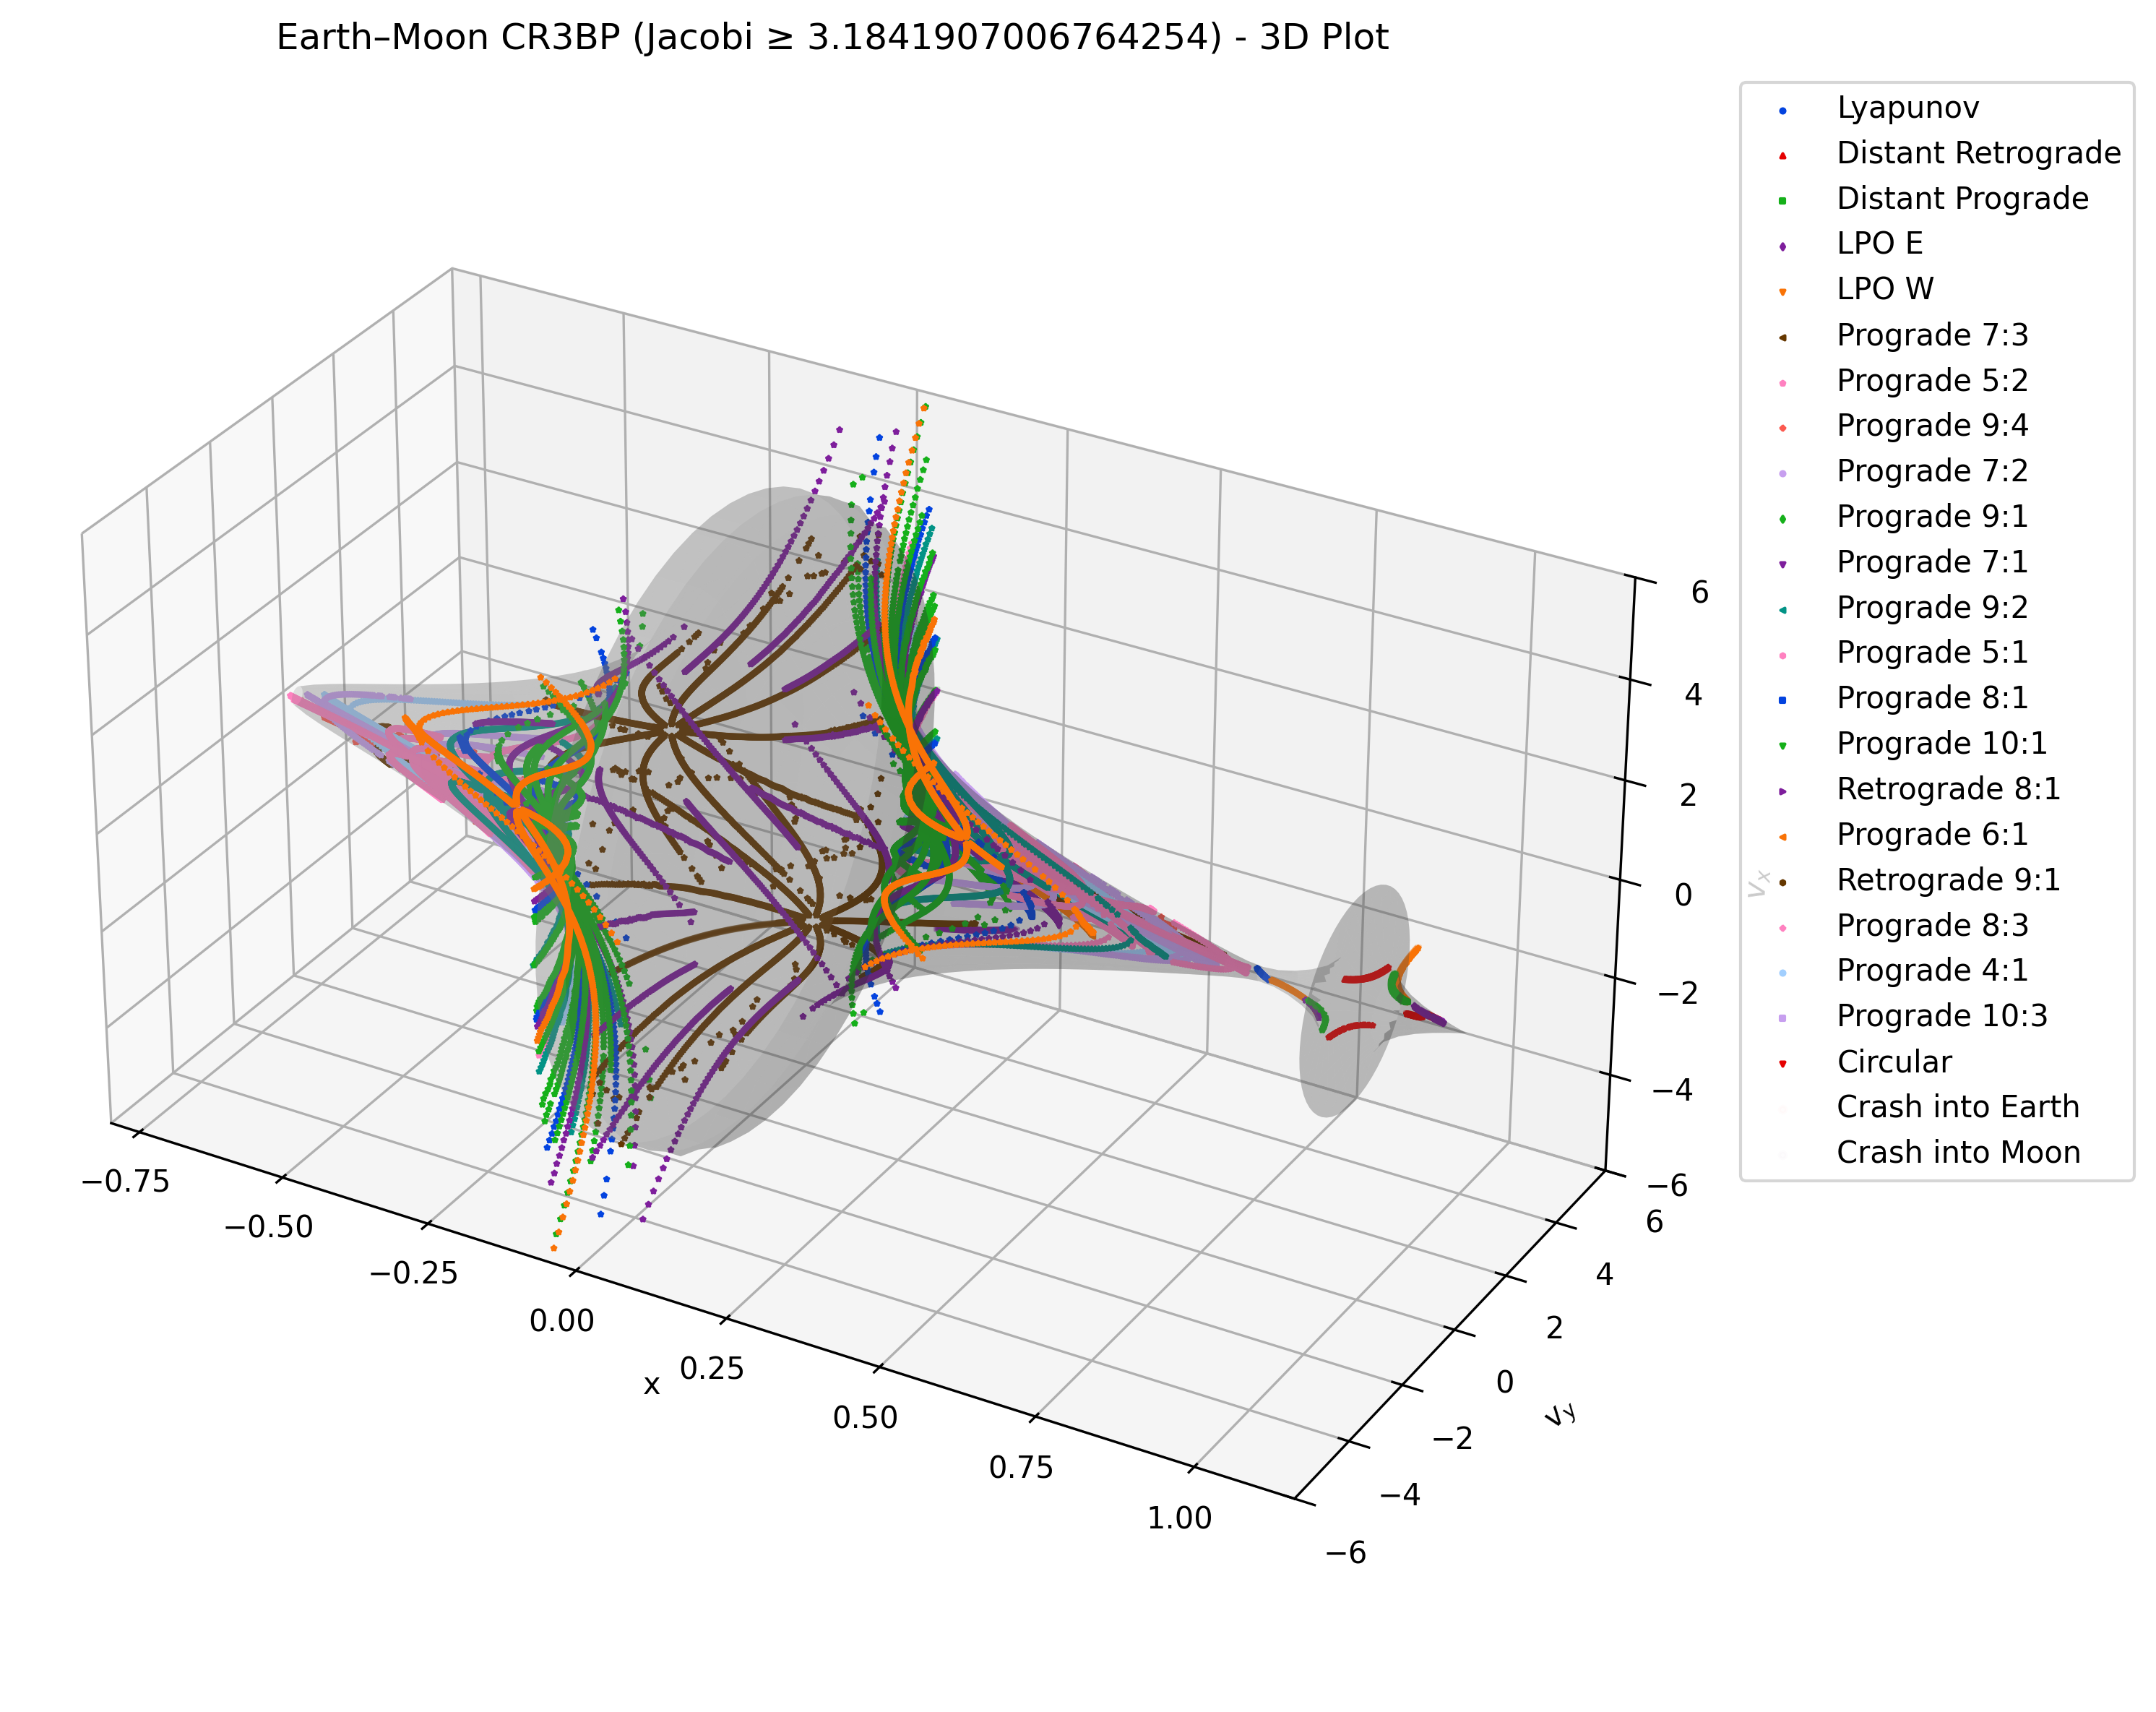
\includegraphics[width=2.9in]{images/3D crossings all orbits.png}
        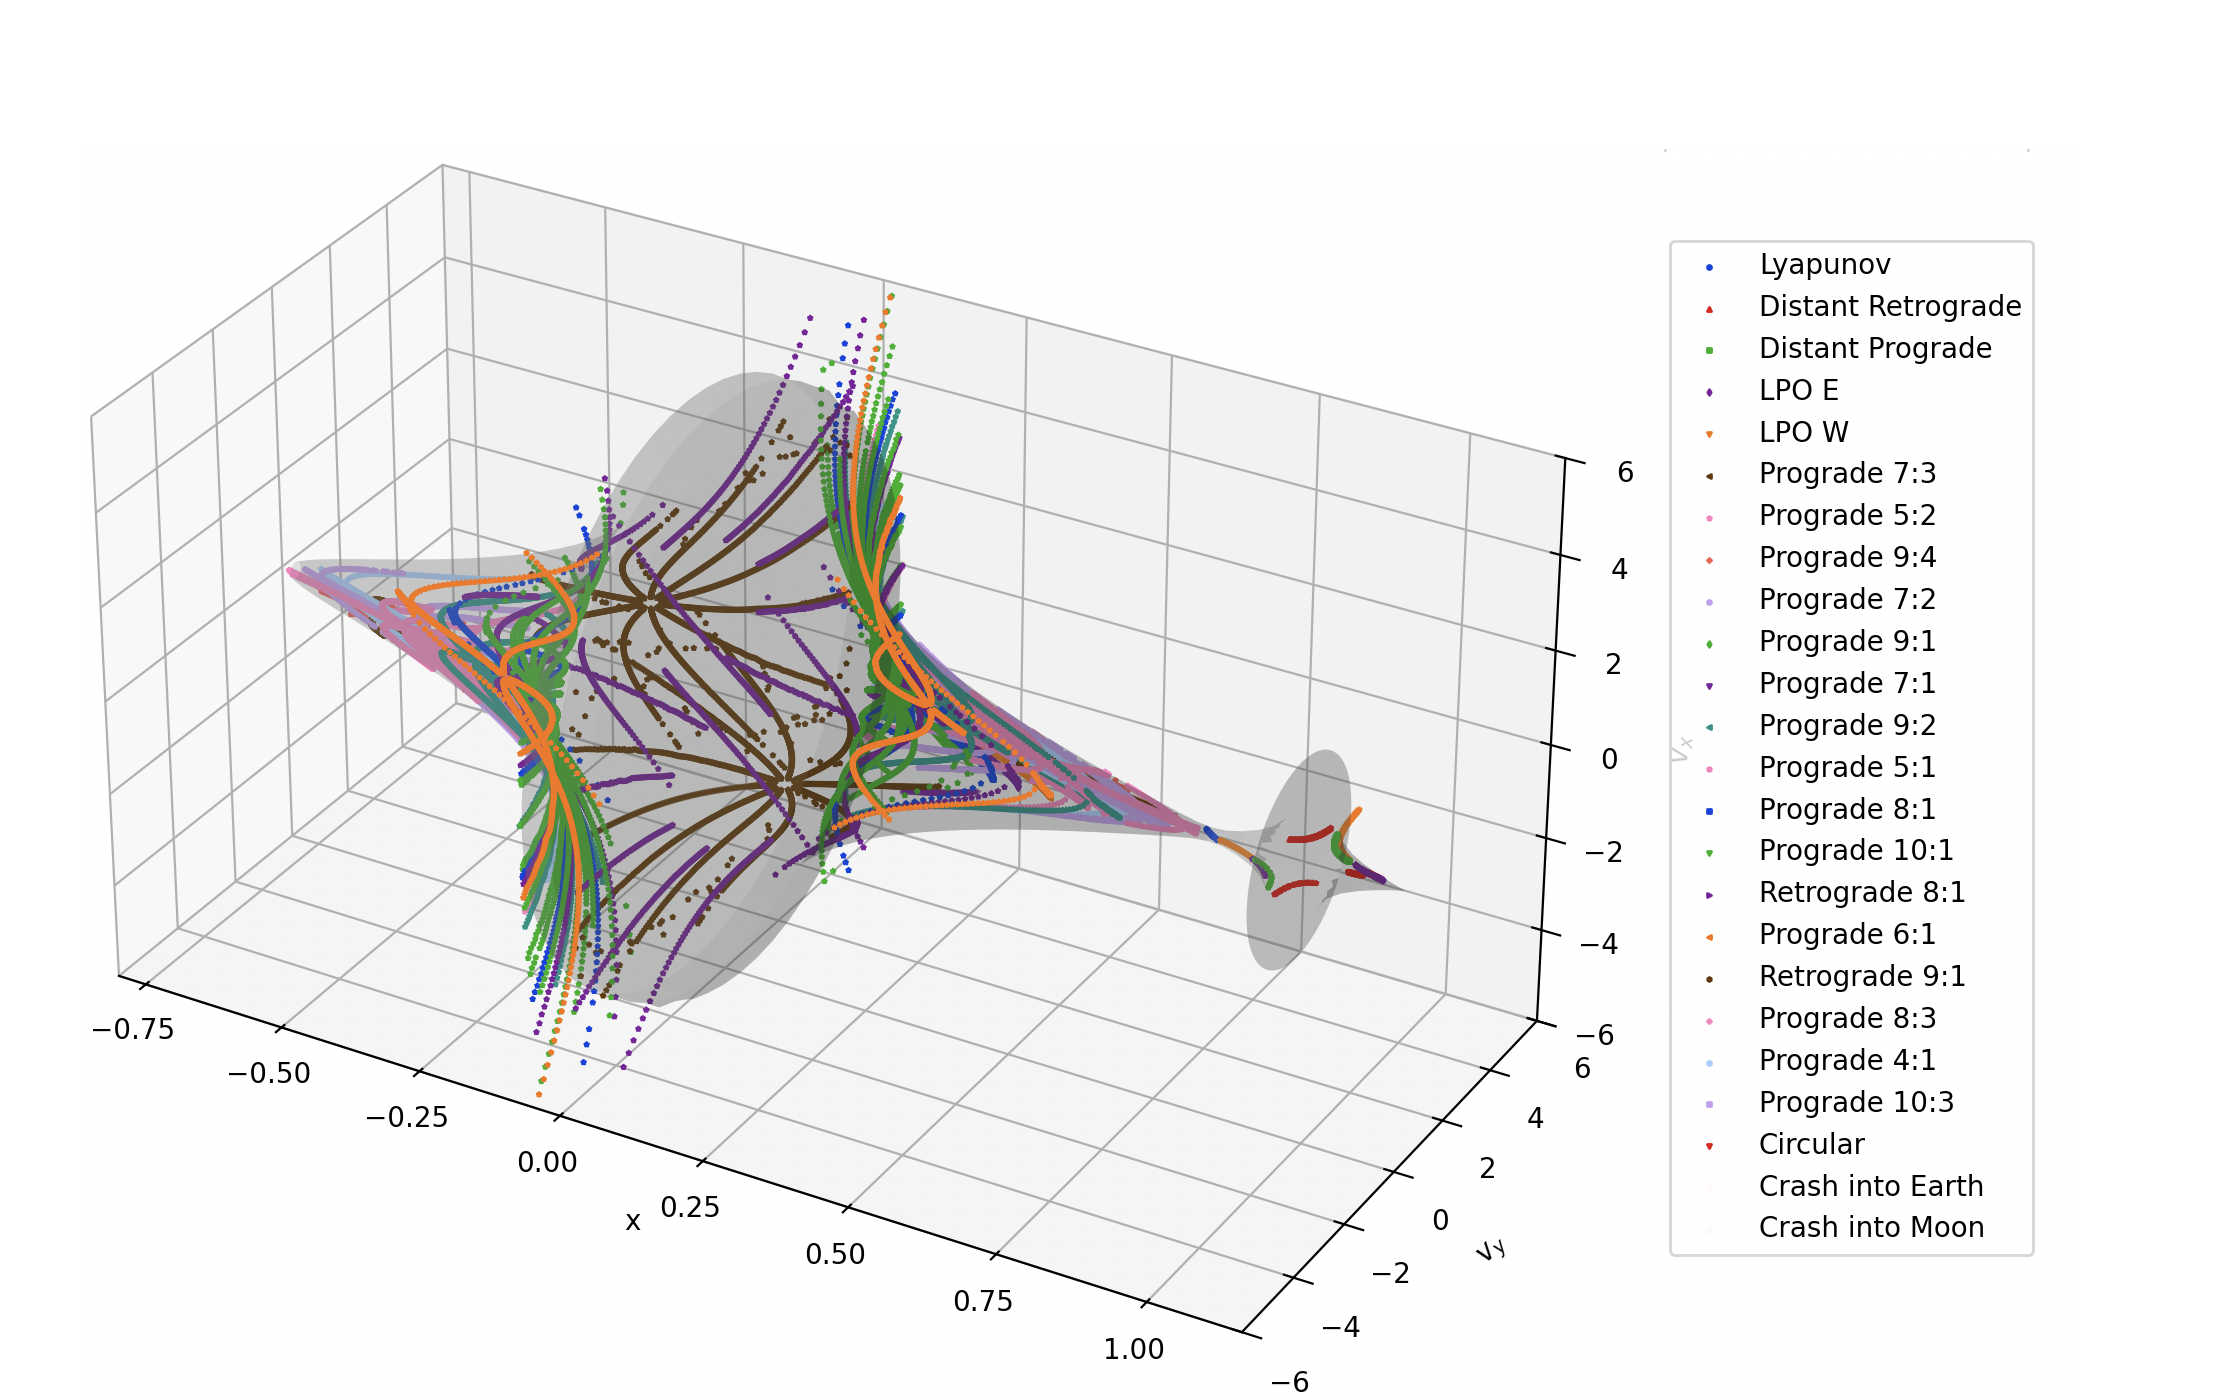
\includegraphics[width=0.85\linewidth]{images/manually made 3d.png}
        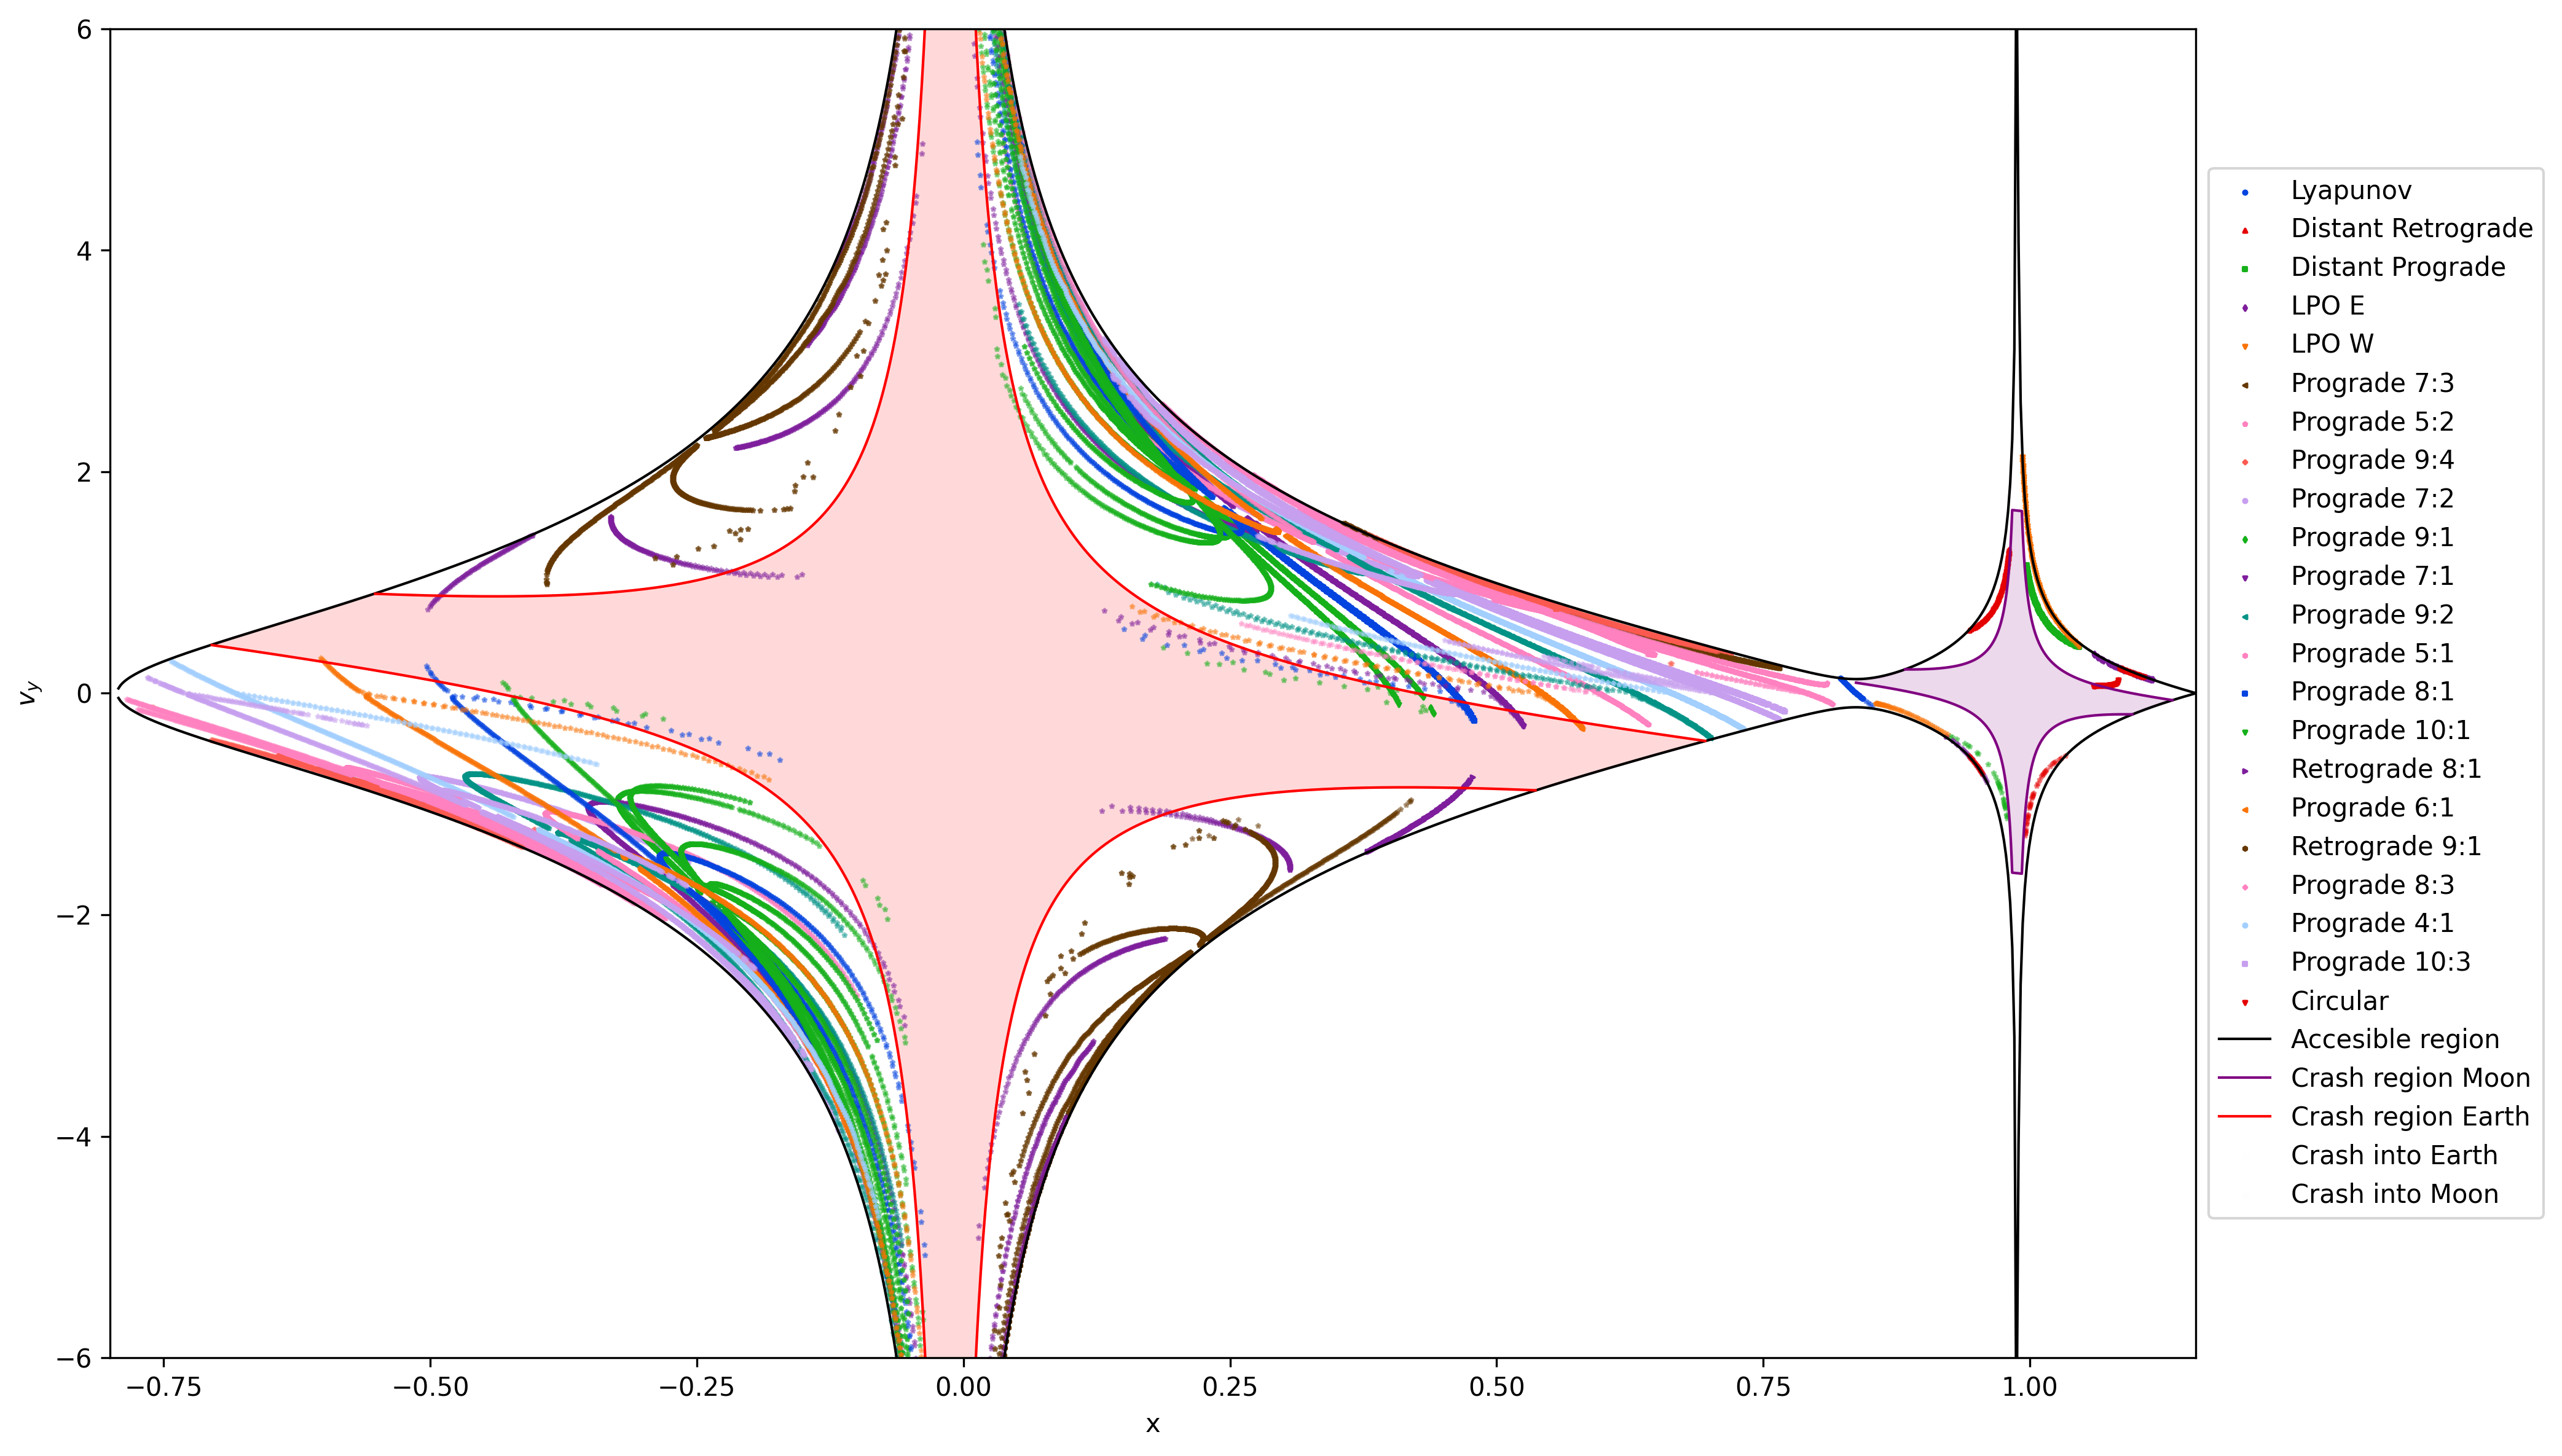
\includegraphics[width=0.75\linewidth]{images/2D crossings all orbits.png}
        % \caption{Visualisations of the accessible region in three dimensions and its projection to the $(x,v_y)$ plane, displaying the Earth and Moon crash regions. The larger `pseudosphere'-esque region corresponds to the region around Earth, and the smaller: that of the Moon.}
        \caption{Orbital crossings of several planar resonant orbits, depicted in three-dimensions and the projection to the $(x,v_y)$ plane.}
        \label{fig: crossings}
    \end{figure}


    

    In \cref{fig: crossings}, these crossings are depicted in the three-dimensional $x,v_x,v_y$ space, as well as in the projection down to the $x,v_y$ plane, for visual clarity. The colours specified in the legend are consistent across both plots. Although it appears as though some points enter the Earth crash region in the 2D image, this is simply a consequence/limitation of the use of projection.
    
    


    
    % \begin{figure}[hb] \label{fig:orbital crossings plotted}
    % 	\centering
    %     % 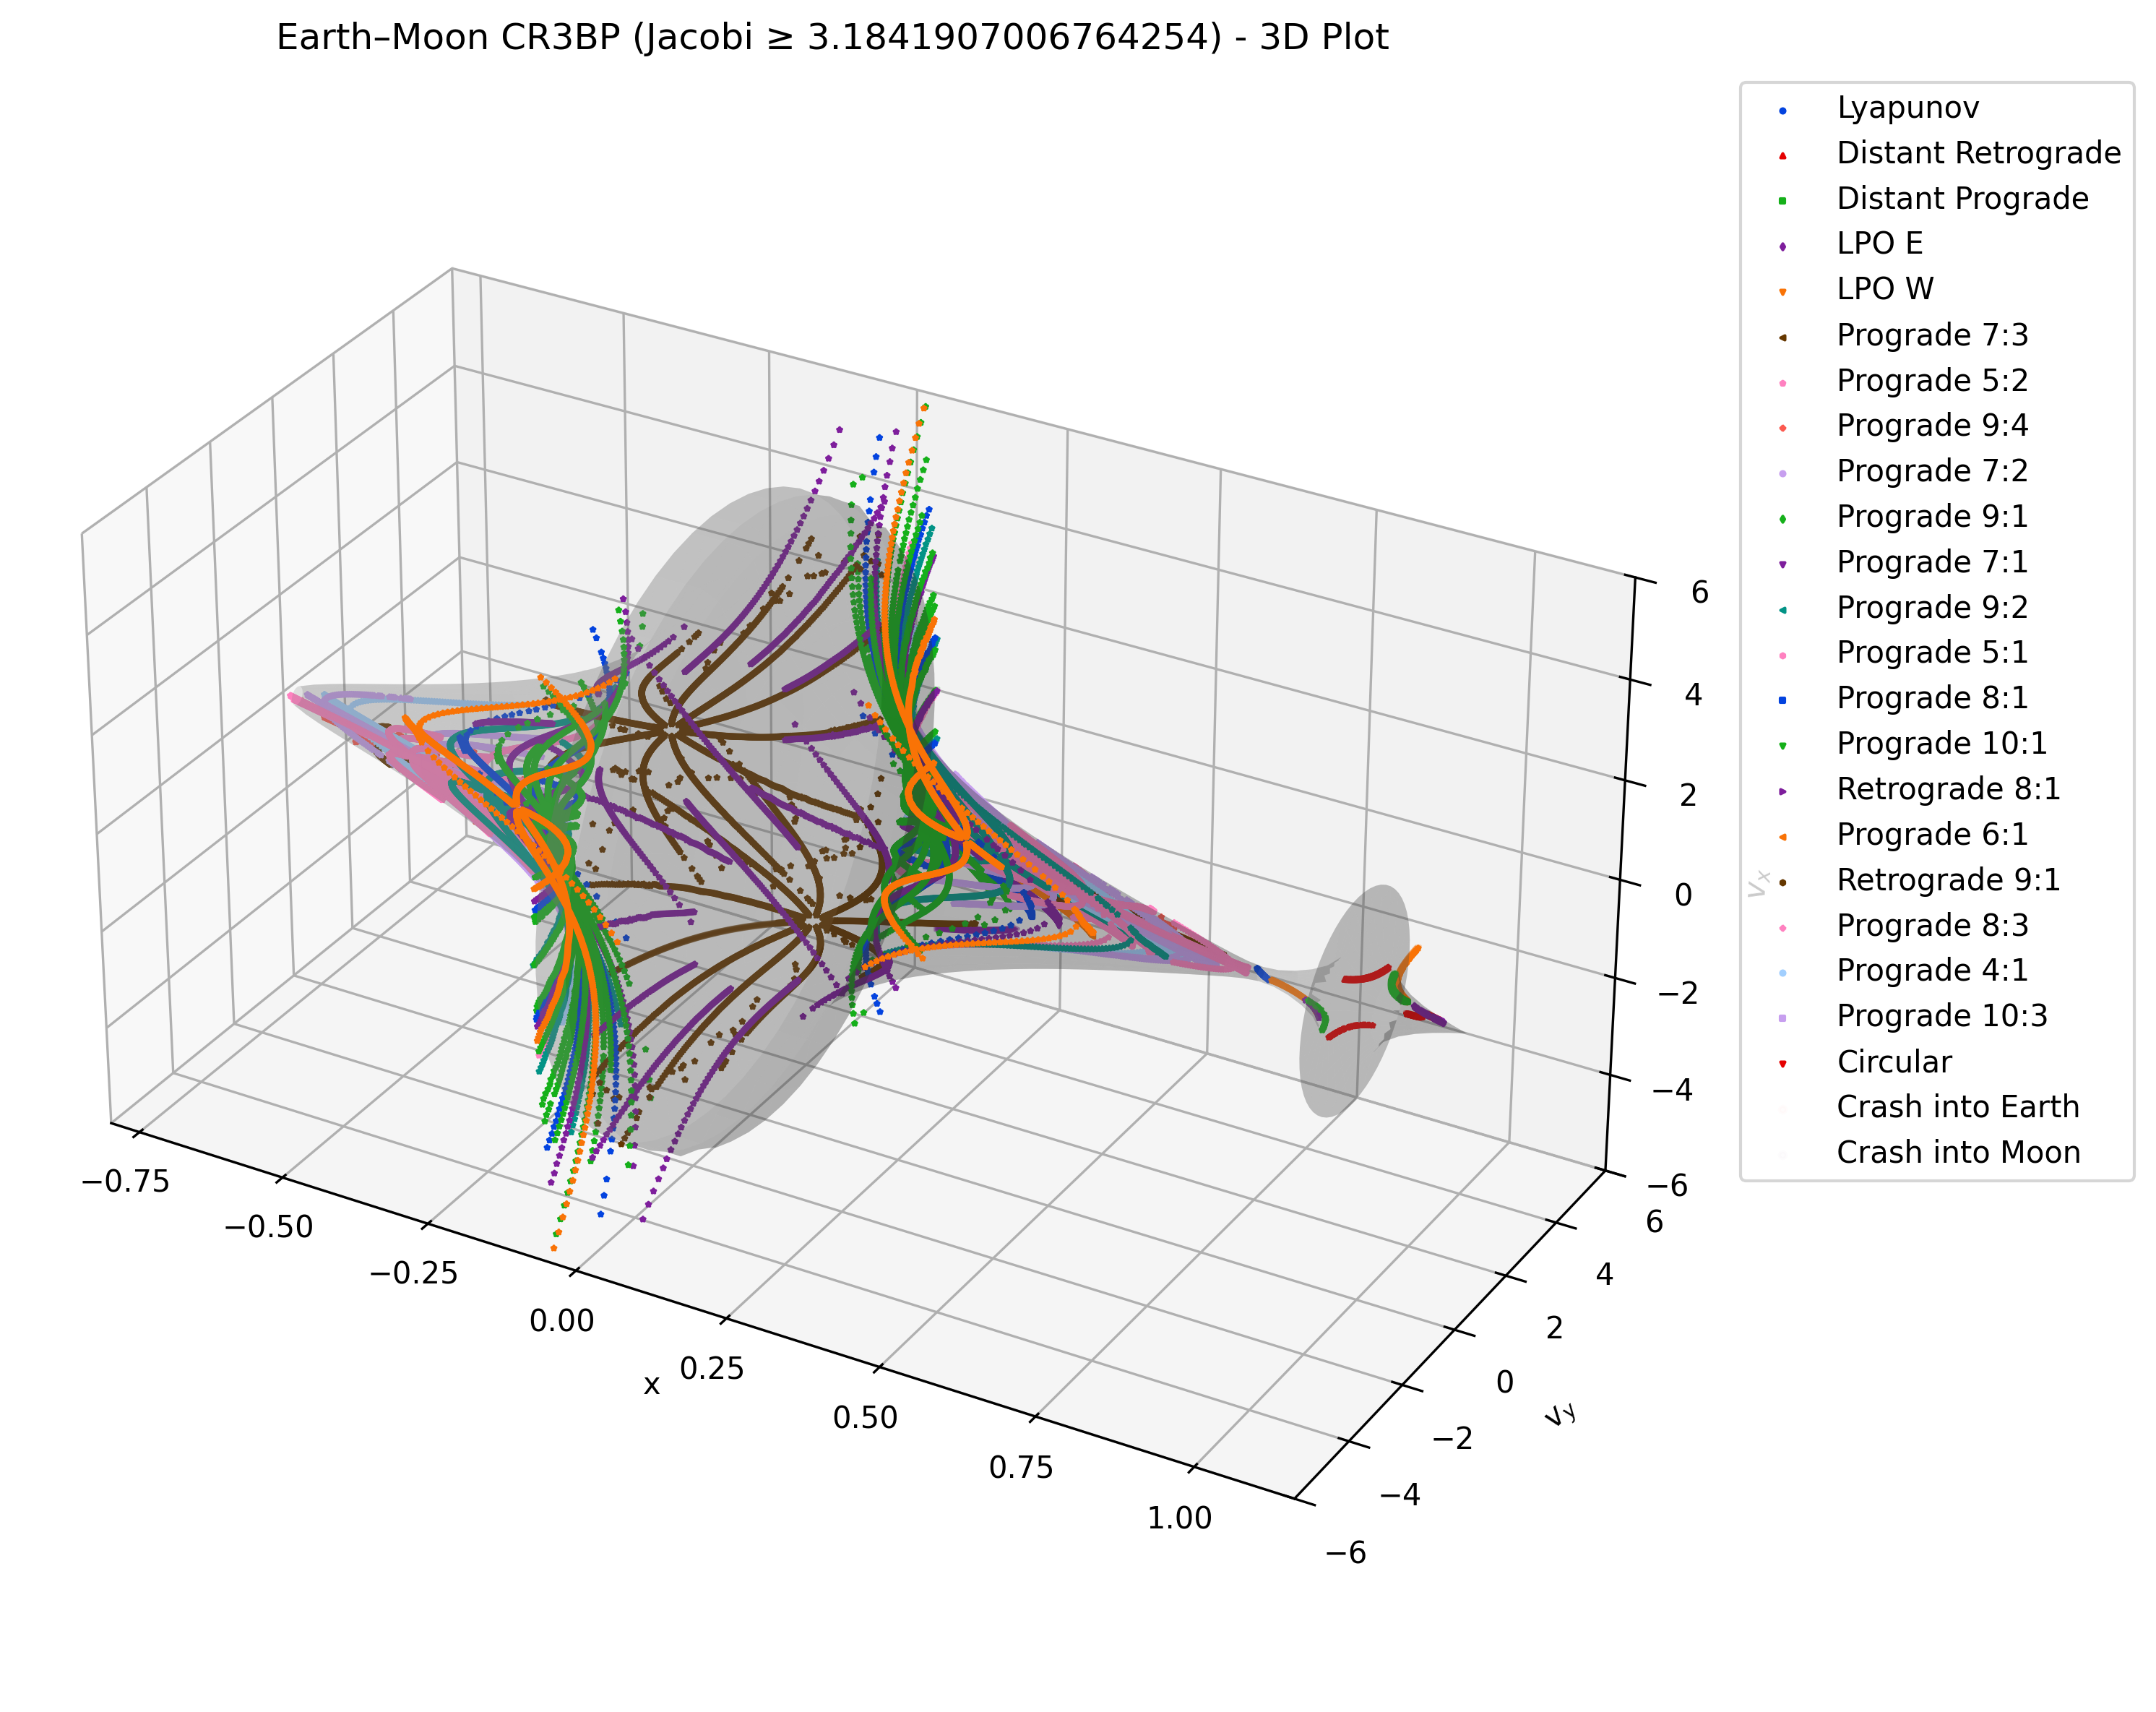
\includegraphics[width=2.9in]{images/3D crossings all orbits.png}
    %     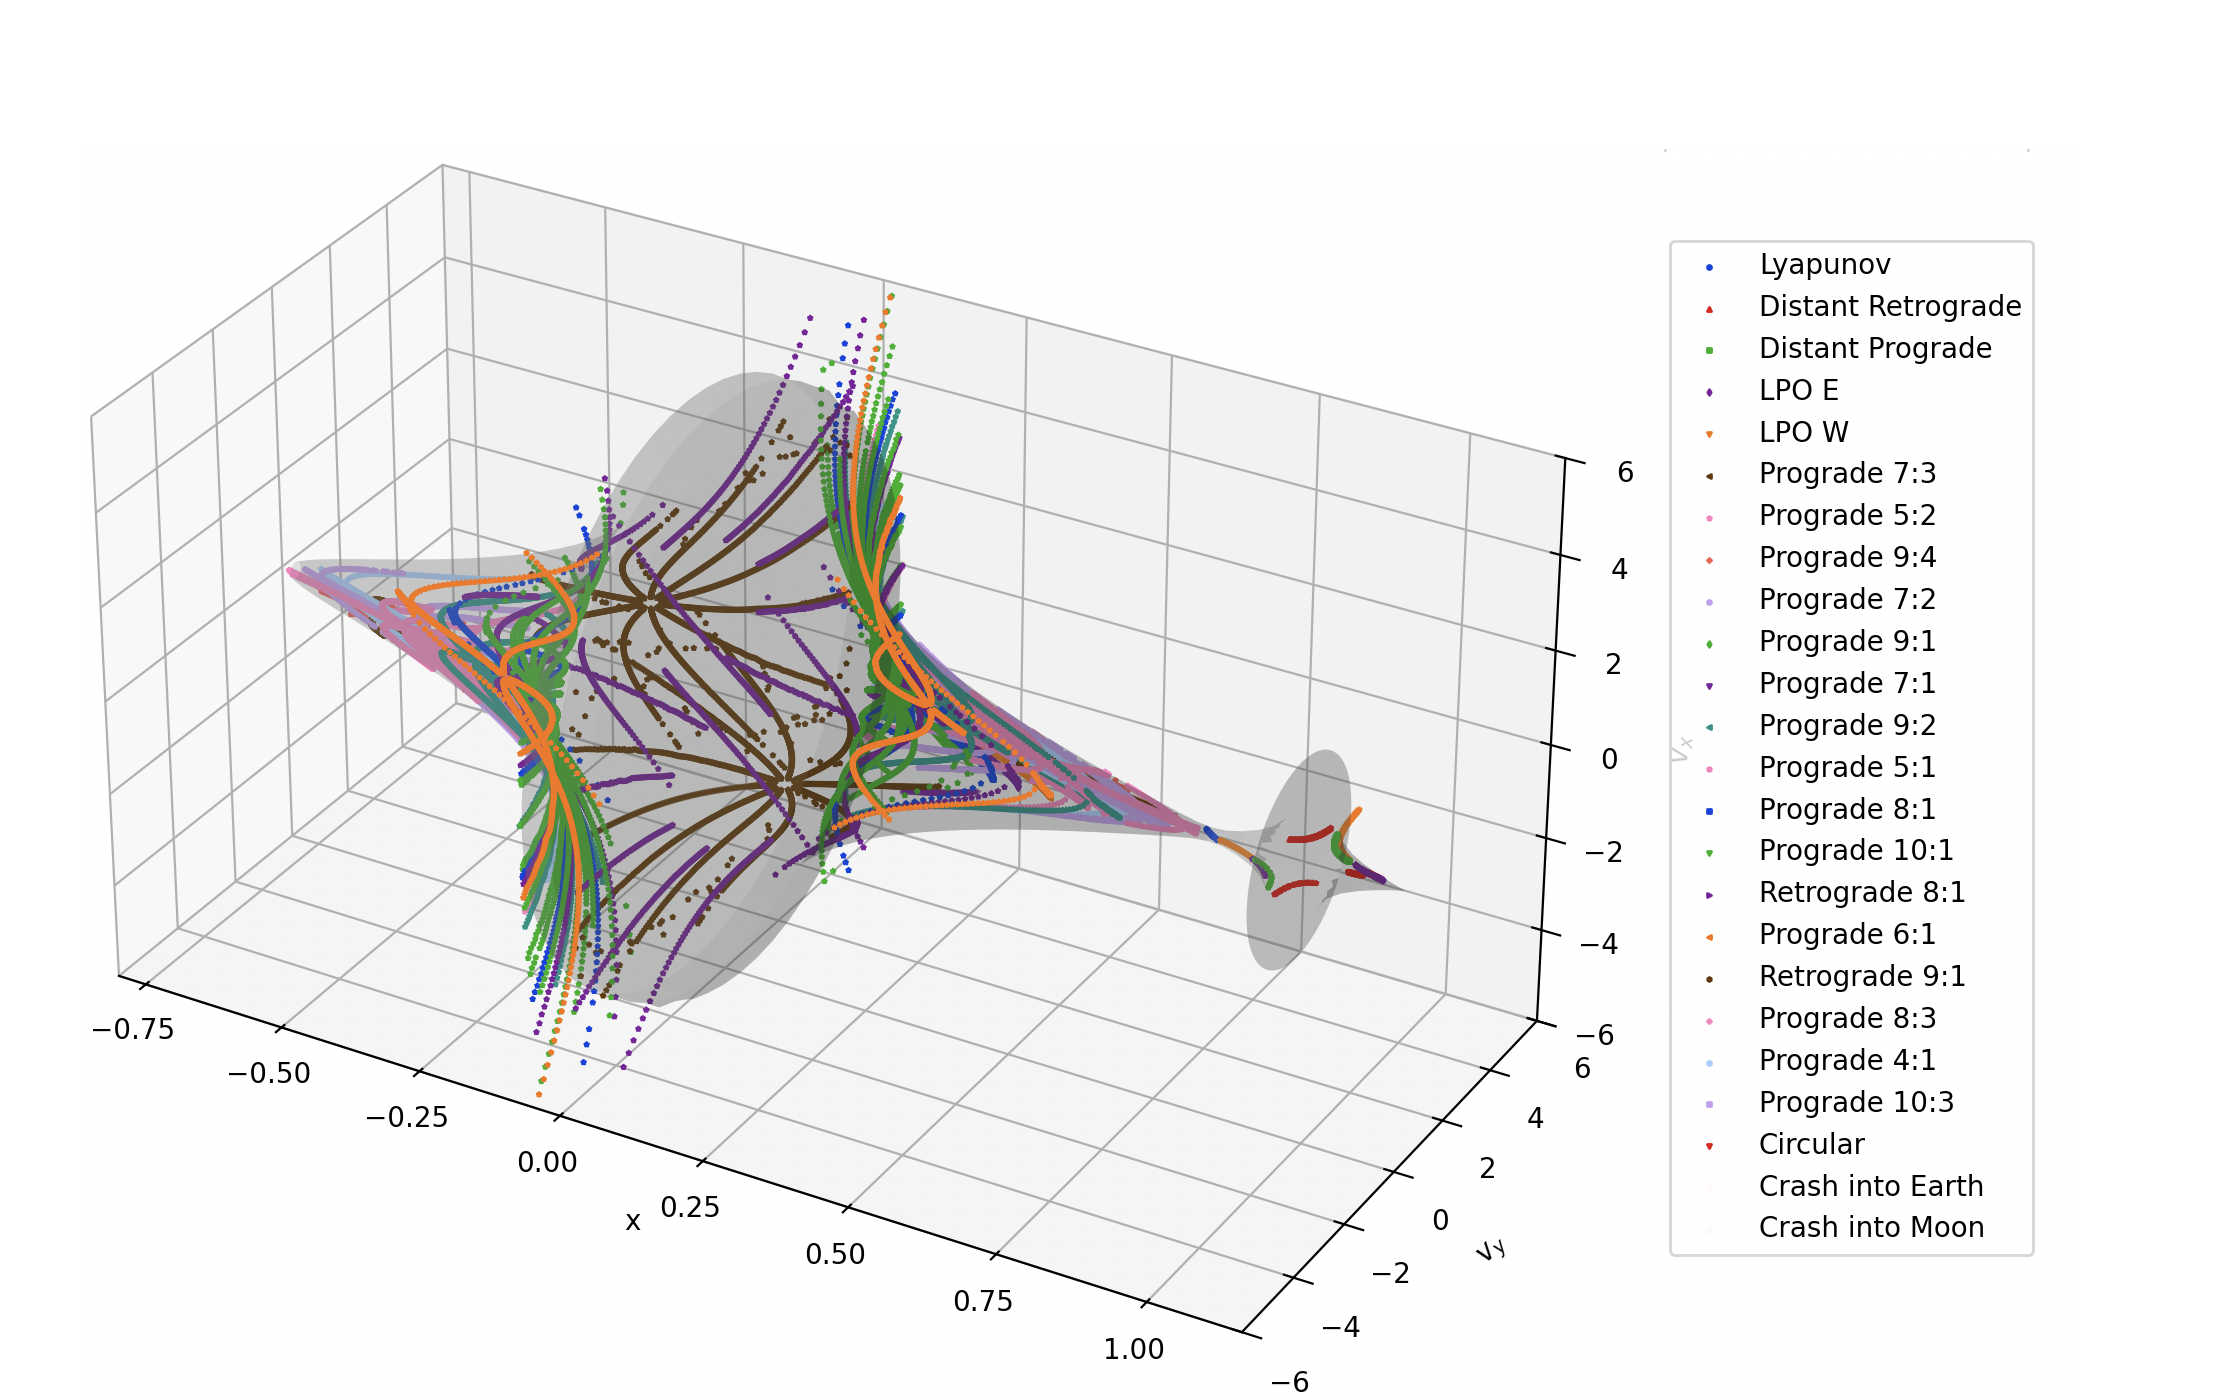
\includegraphics[width=0.85\linewidth]{images/manually made 3d.png}
    %     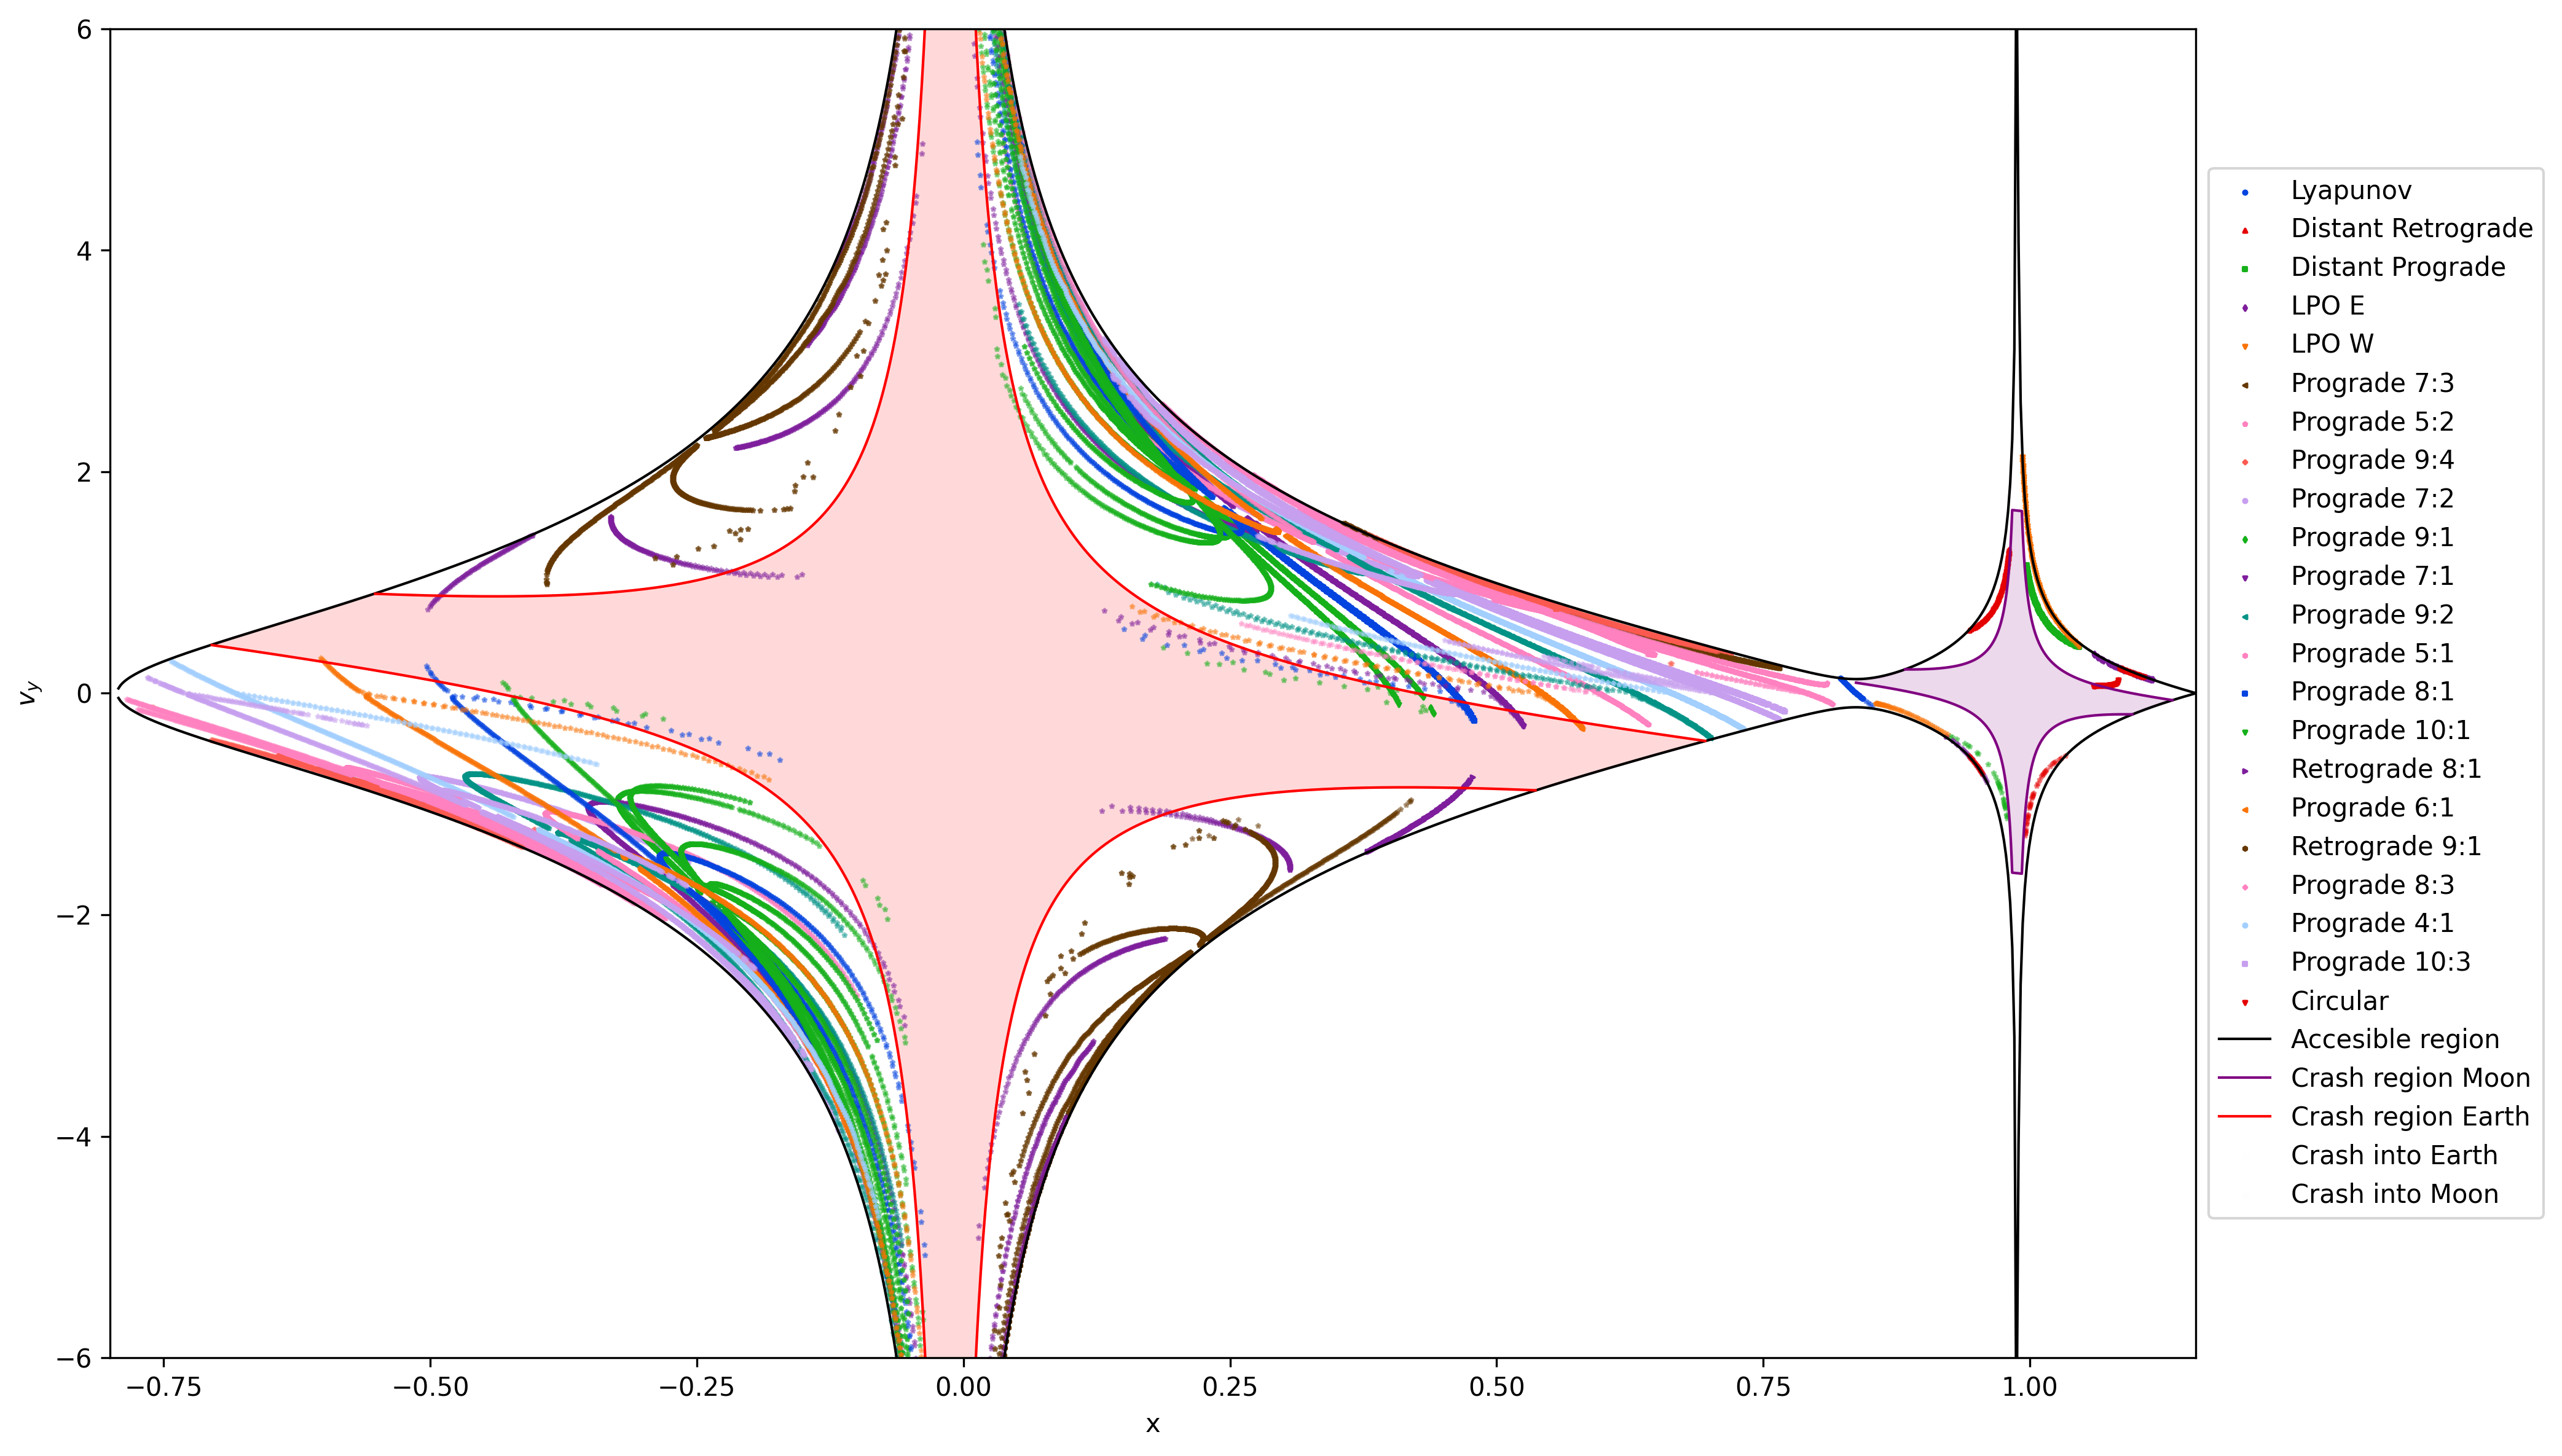
\includegraphics[width=0.75\linewidth]{images/2D crossings all orbits.png}
    %     % \caption{Visualisations of the accessible region in three dimensions and its projection to the $(x,v_y)$ plane, displaying the Earth and Moon crash regions. The larger `pseudosphere'-esque region corresponds to the region around Earth, and the smaller: that of the Moon.}
    %     \caption{Orbital crossings of several planar resonant orbits, depicted in three-dimensions and the projection to the $(x,v_y)$ plane.}
    %     \label{fig: crossings}
    % \end{figure}



    Ultimately, an interesting direction for future work may be investigating the `coverage' of these crossings within our accessible region, potentially finding a method to cover the space with such points to an arbitrary degree.


    Such an effort is not unfounded, results by Poincaré in \cite{Poincare_1893} following a conjecture in \cite{Poincare_1892}, demonstrate the density of periodic orbits at least in analogous, low-energy regimes. It has not been ruled out, and is viewed as likely by the authors and by a larger portion of the astrodynamics community, that this density of periodic orbits may extend to our domain as well.

    Regardless, as can be seen in \cref{fig: crossings}, at least with the families of orbits tested, we have struggled to find families with many crossings close to the inner portion or the space/near the crash region. (Qualitatively, one can see that the points plotted are much more `dense' near the boundary of the accessible region. This is at least true when viewing the upper right and lower left quadrants, as these house the crossings of prograde orbits, which are much more numerous in our tested families due to data availability/the data we computed. Not much should be read into the sparsity of points in the upper left and lower right quadrants (and lunar region), for this reason.)






    \subsection{Chaos in the Cross-Sections}


    In the following \cref{fig: constant energy Poincaré sections}, we briefly provide depictions of the chaos apparent in our system by viewing the action of the Poincaré map on various initial points each with varying colour based on initial location.    
    
    These depictions are done on several Poincaré sections, using the Jacobi constant, $C$, as a proxy for energy. One can see that for $C$ closer to $3.2$, approximately the Jacobi constant correlating to $E_2$ (recall \cref{eq: energy E2}, and that $C = -2E$), the chaotic nature of the system becomes increasingly prominent.
    

    \begin{figure}[h]
        \centering
        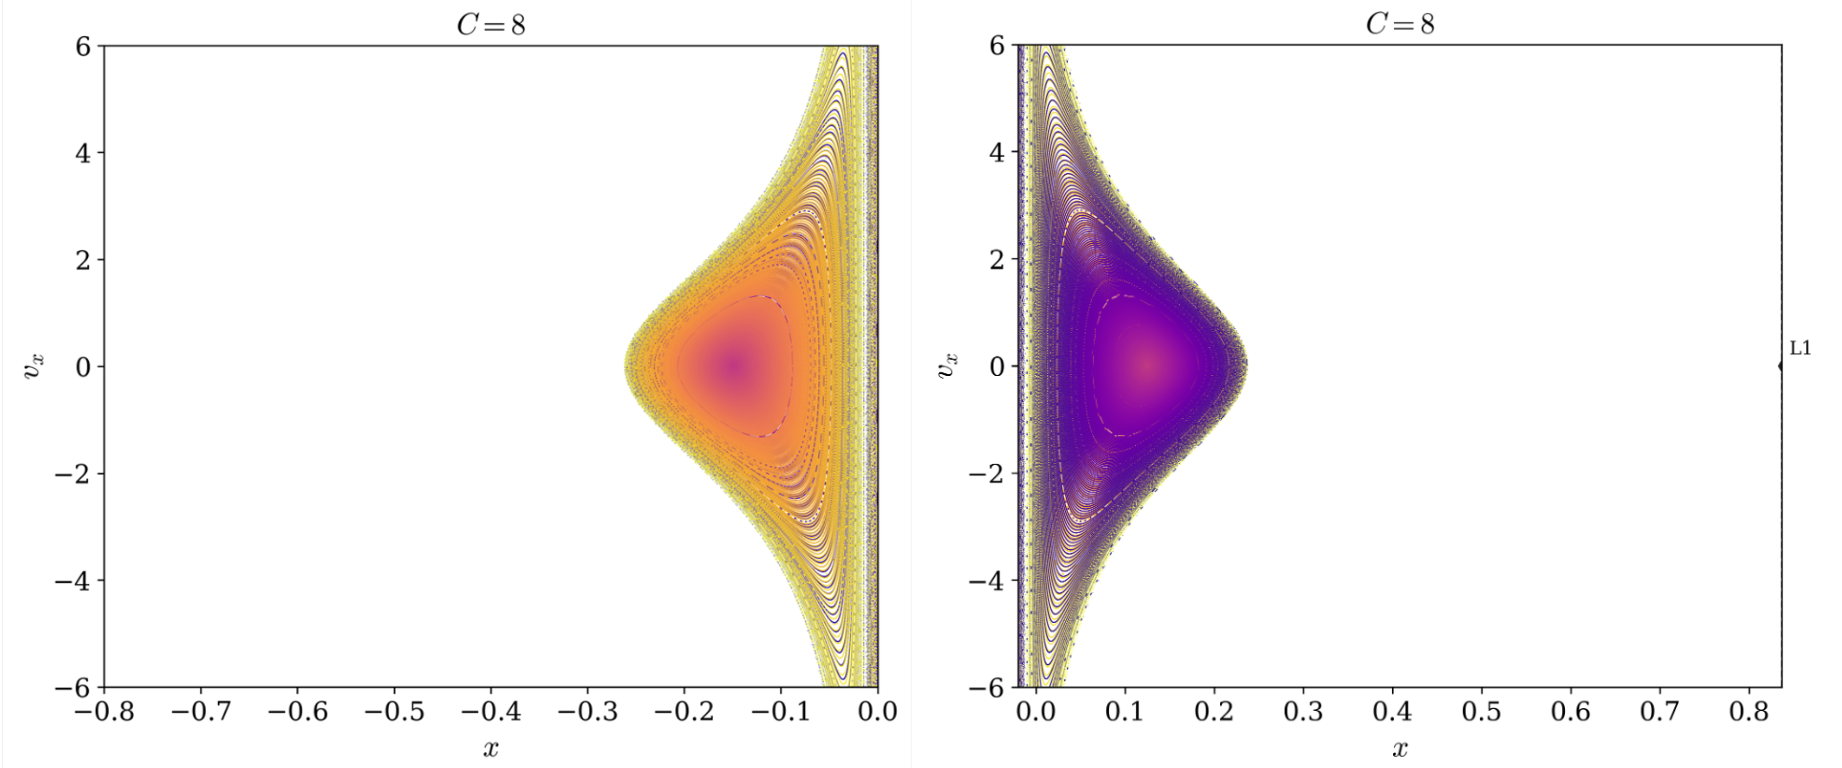
\includegraphics[width=1\linewidth]{images/chaos C 8 .png}
        % 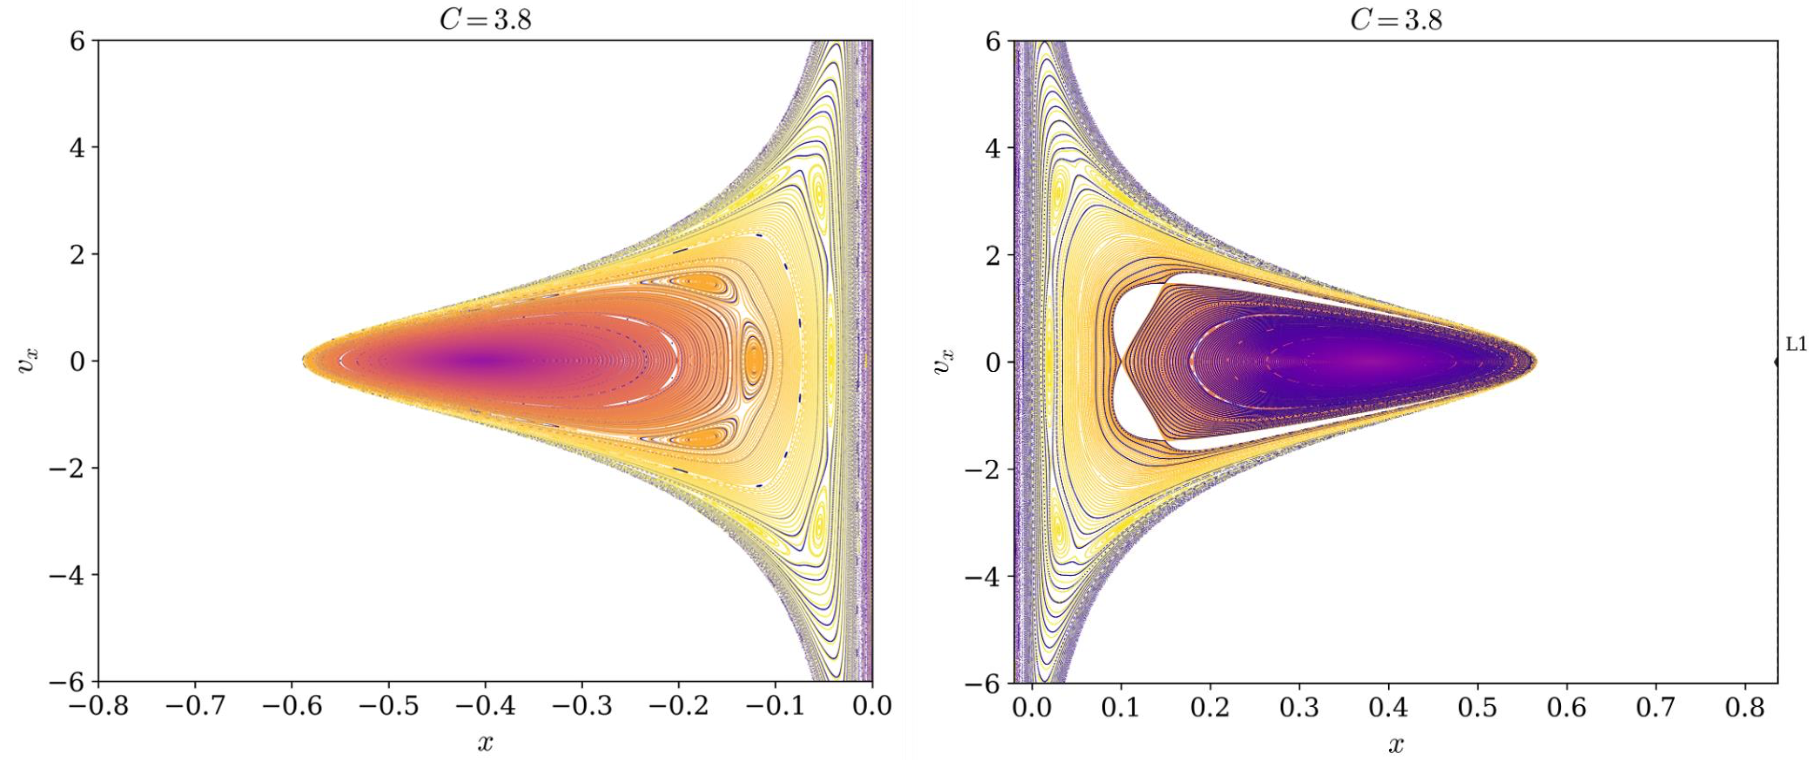
\includegraphics[width=1\linewidth]{images/chaos C 3.8 .png}
        % 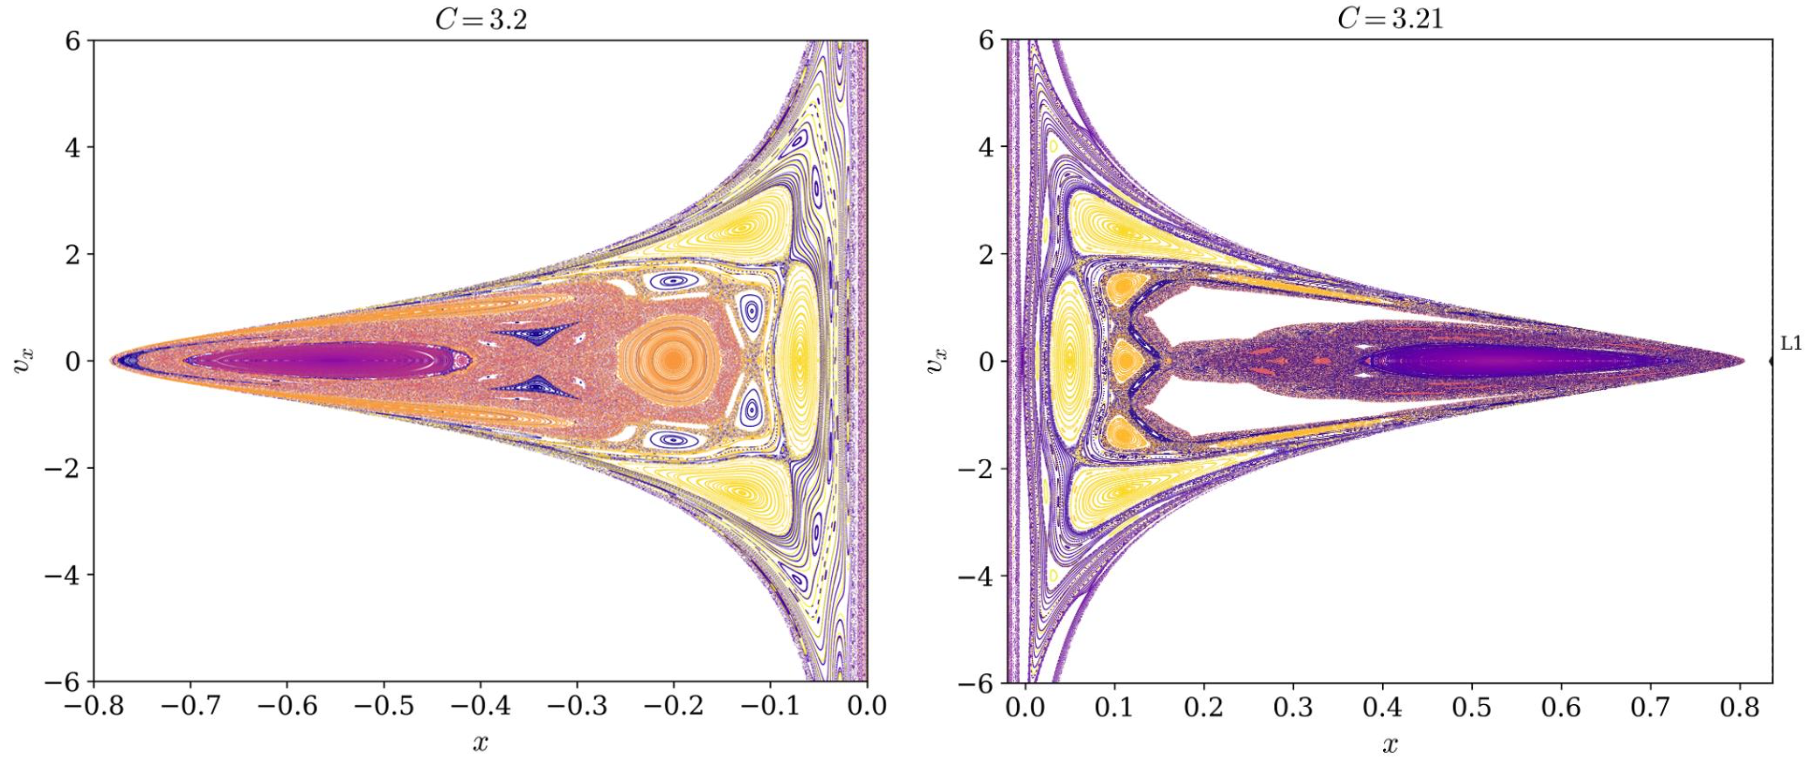
\includegraphics[width=1\linewidth]{images/chaos C 3.2 .png}
        \caption{Poincaré sections for different Jacobi constants.}
        \label{fig: constant energy Poincaré sections}
    \end{figure}

    
    \begin{figure}[h]
        \centering
        % 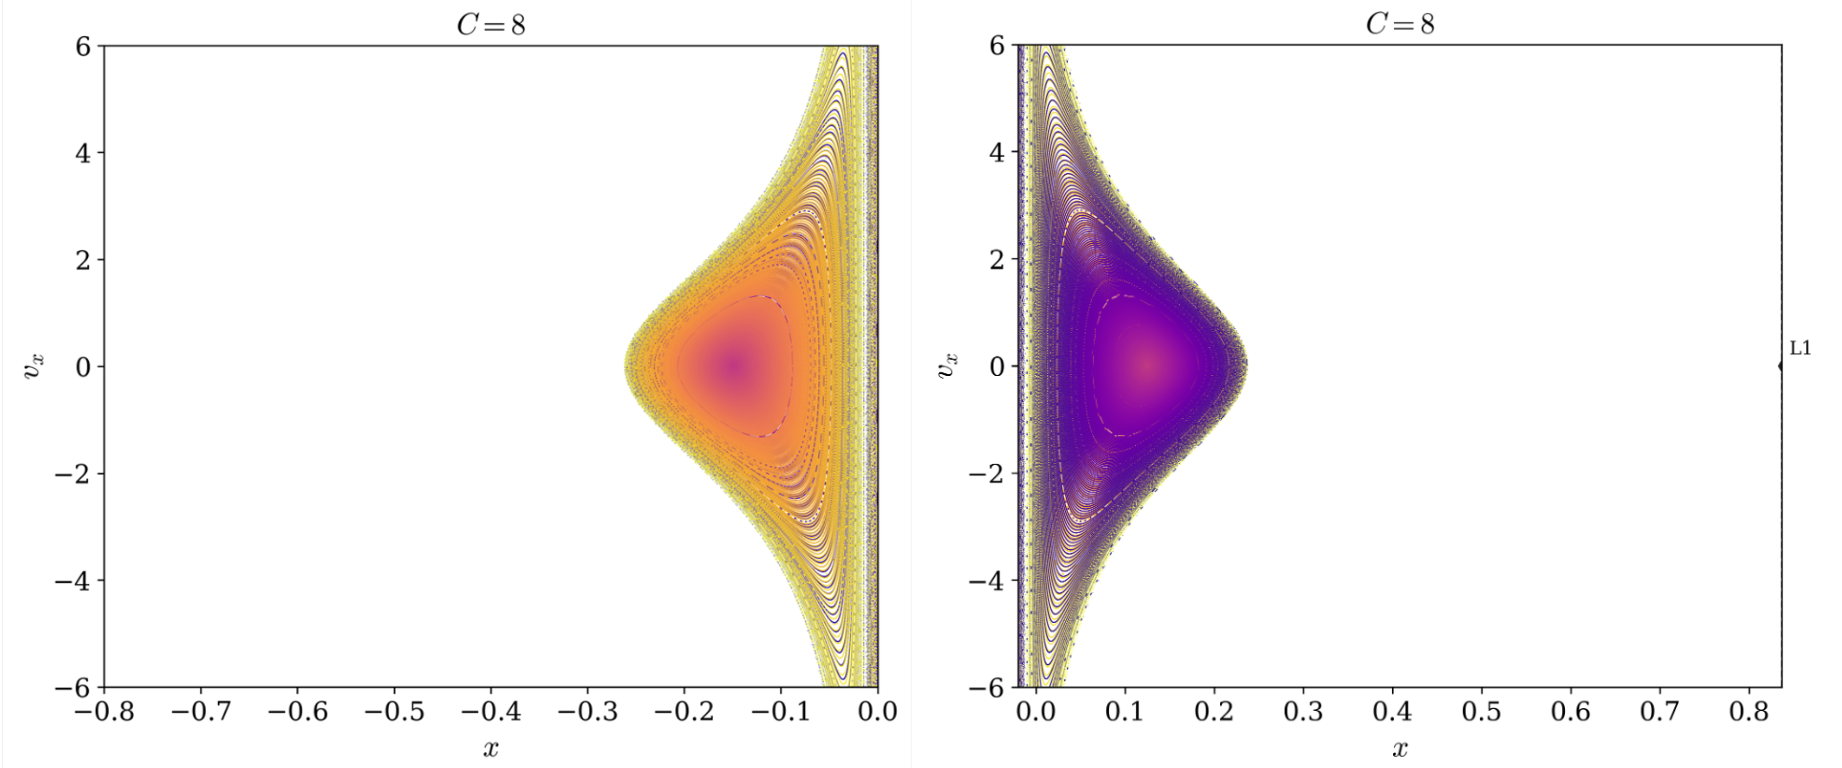
\includegraphics[width=1\linewidth]{images/chaos C 8 .png}
        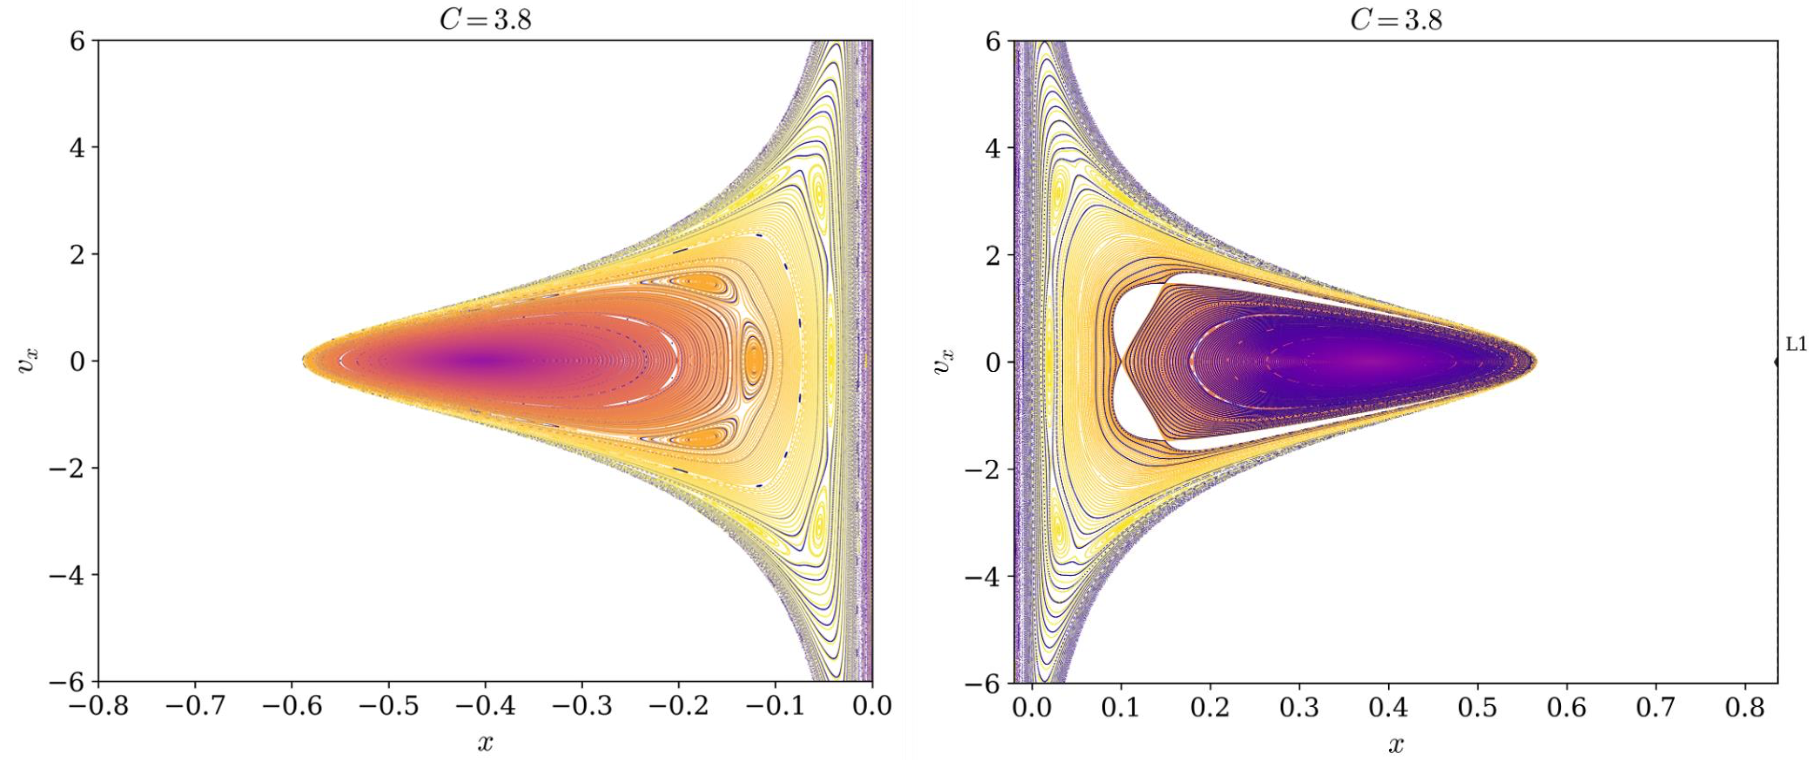
\includegraphics[width=0.81\linewidth]{images/chaos C 3.8 .png}
        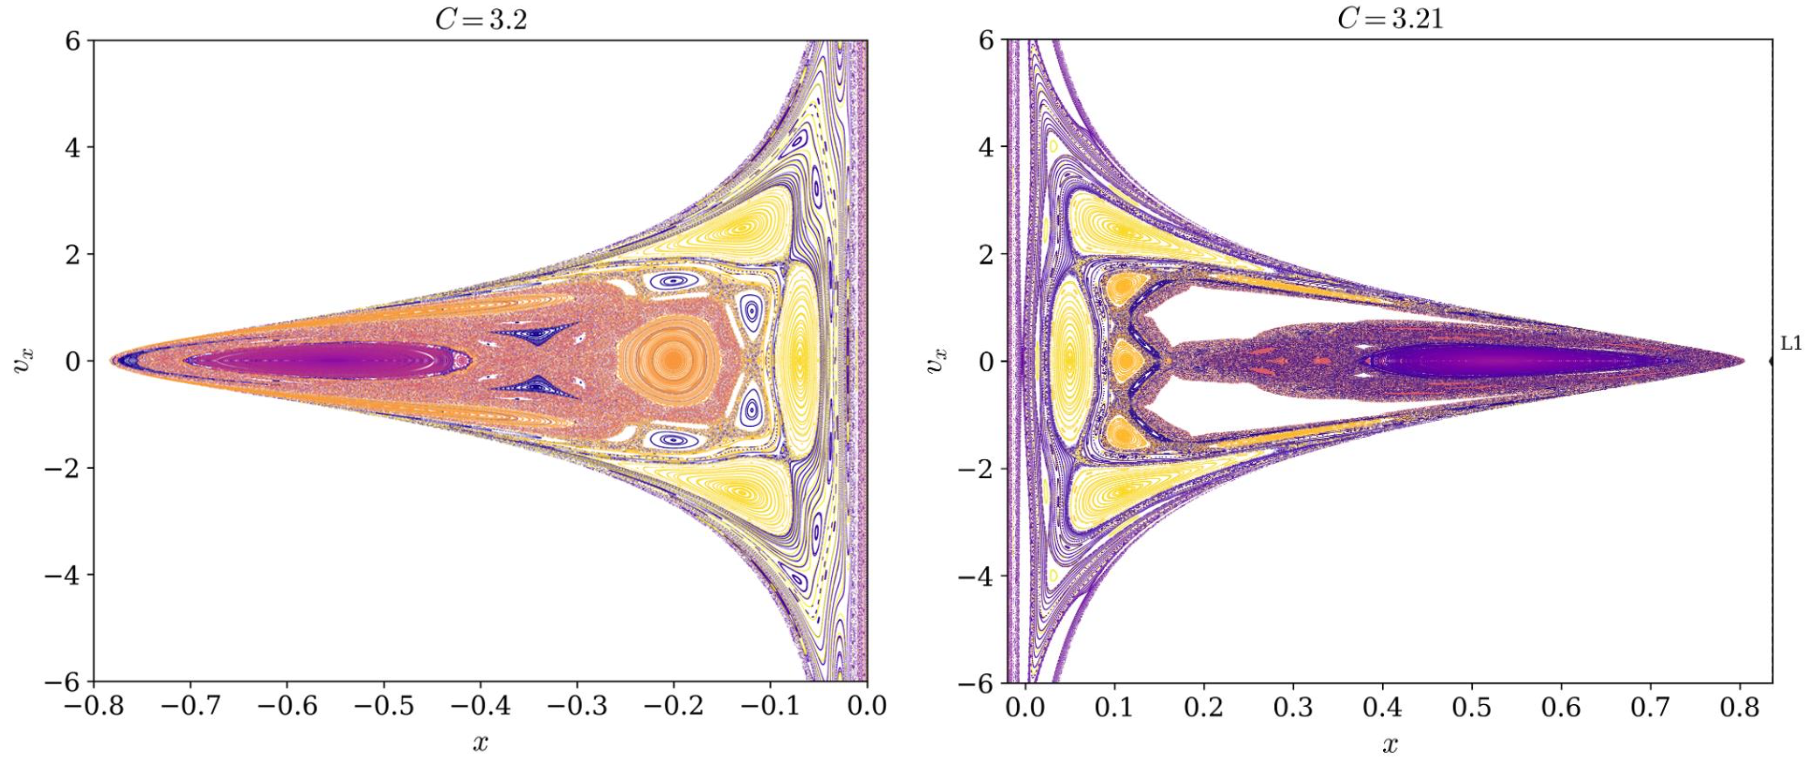
\includegraphics[width=0.81\linewidth]{images/chaos C 3.2 .png}
        % \label{fig: constant energy Poincaré sections}
    \end{figure}



    % \begin{figure}[h]
    %     \centering
    %     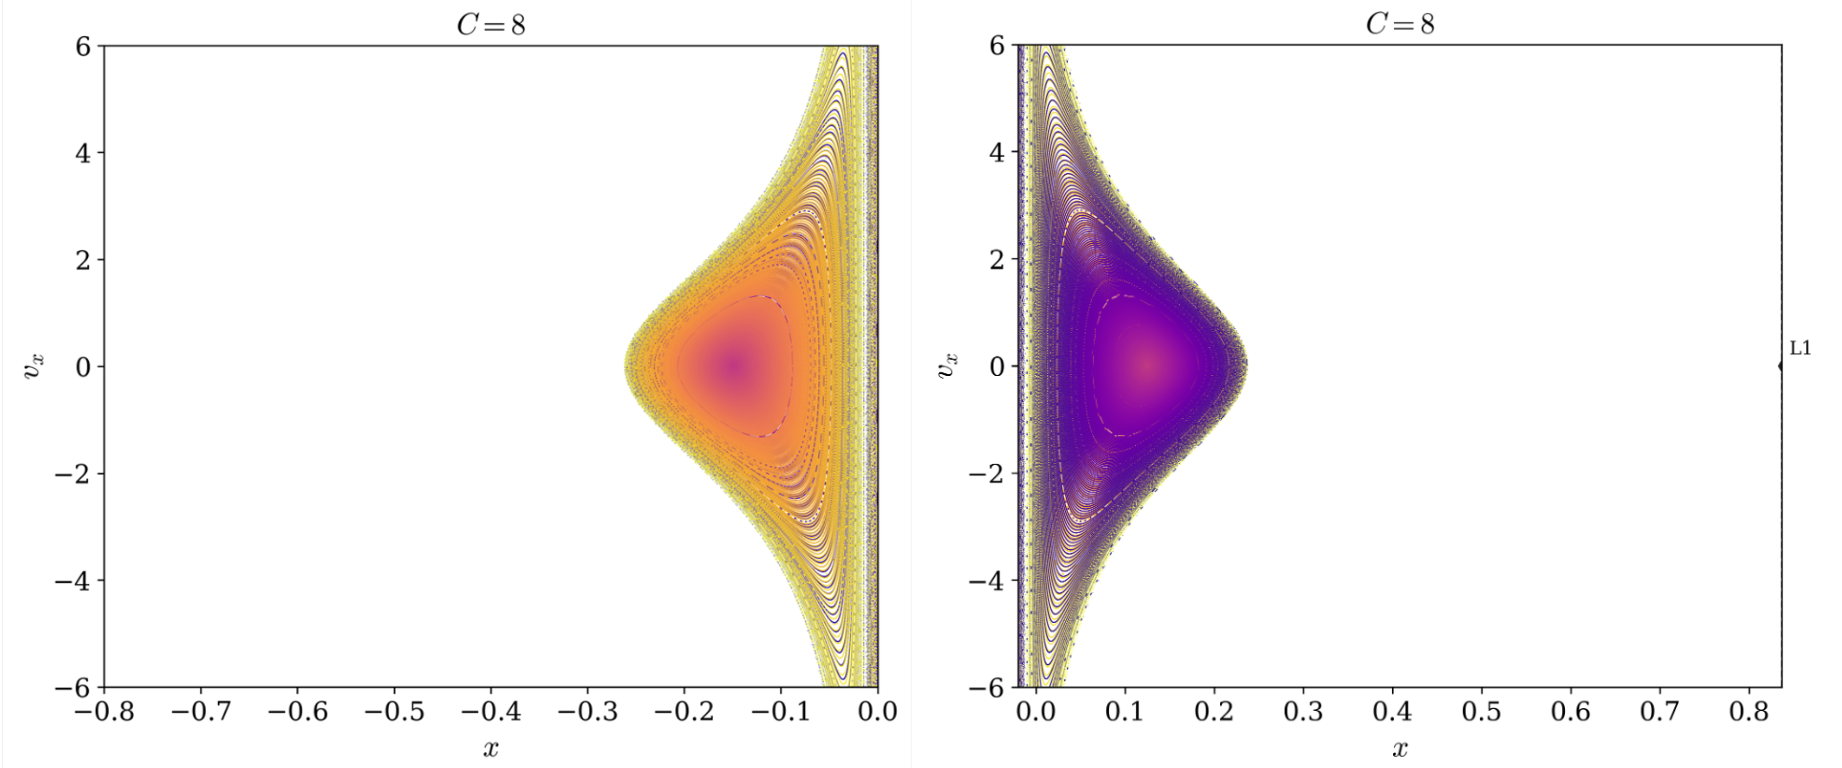
\includegraphics[width=0.8\linewidth]{images/chaos C 8 .png}
    %     % \caption{Poincaré sections for constant Jacobi constants.}
    %     % \label{fig: constant energy Poincaré sections}
    % \end{figure}
    
    % \begin{figure}[h]
    %     \centering
    %     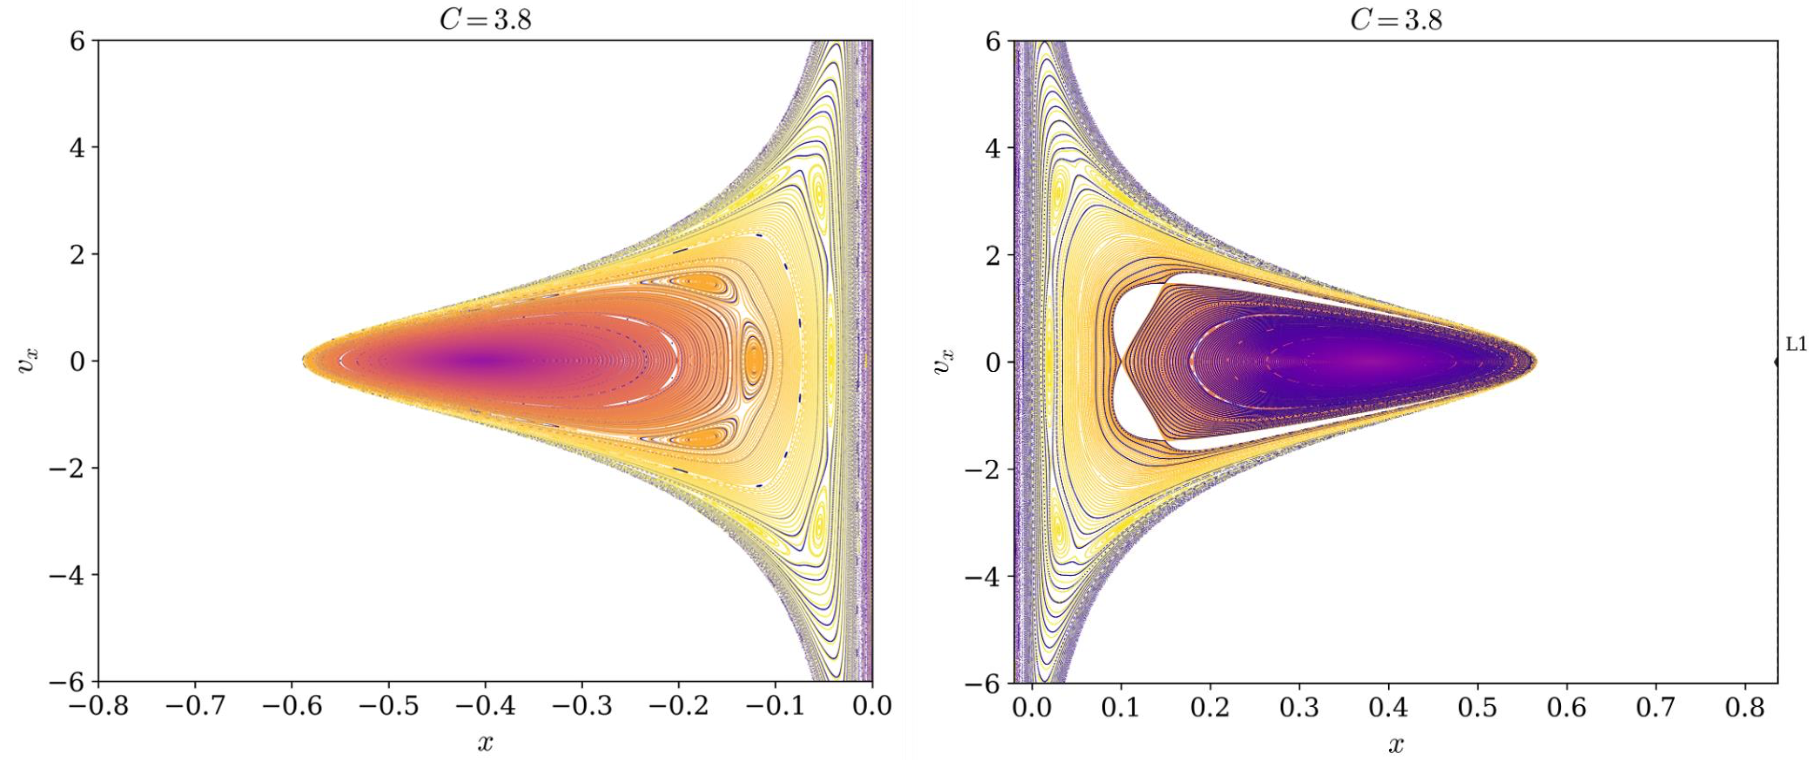
\includegraphics[width=0.8\linewidth]{images/chaos C 3.8 .png}
    %     % \caption{Poincaré sections for constant Jacobi constants.}
    %     % \label{fig: constant energy Poincaré sections}
    % \end{figure}

    % \begin{figure}[h]
    %     \centering
    %     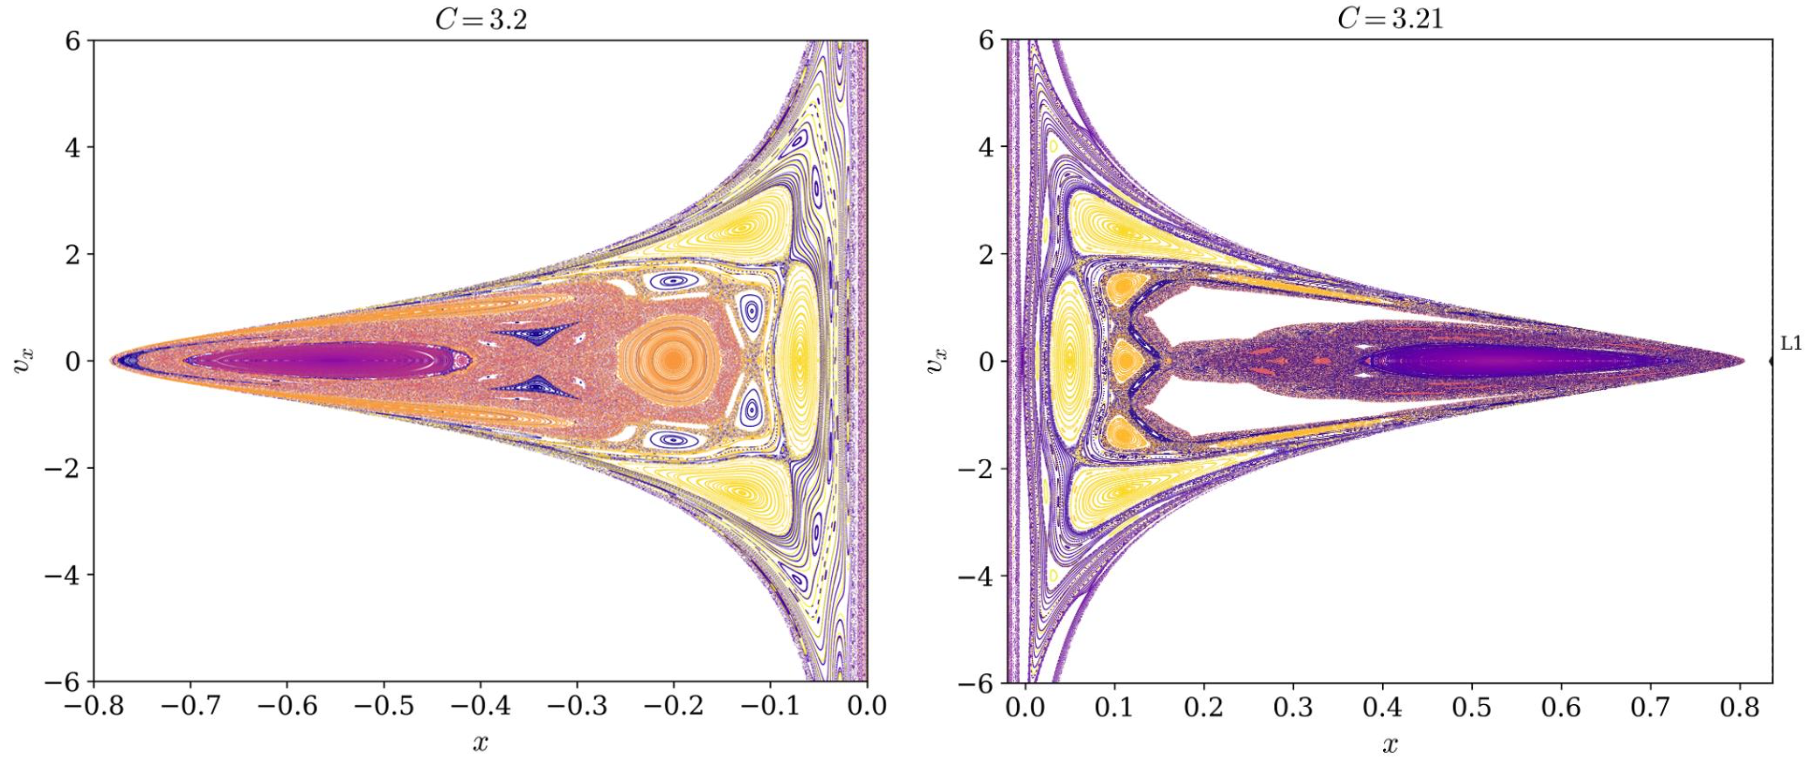
\includegraphics[width=0.8\linewidth]{images/chaos C 3.2 .png}
    %     % \caption{Poincaré sections for constant Jacobi constants.}
    %     % \label{fig: constant energy Poincaré sections}
    % \end{figure}





    Further, the large `islands of stability', prominent in \cref{fig: constant energy Poincaré sections} and characterised by concentric rings, are nicely centred around low ratio $p:q$ resonant orbits. \cref{fig: Jannik's nice poincare pq diagram} provides a particularly enlightening depiction of several of these points.

    \vspace{1cm}

    \begin{figure}[hbt]
        \centering
        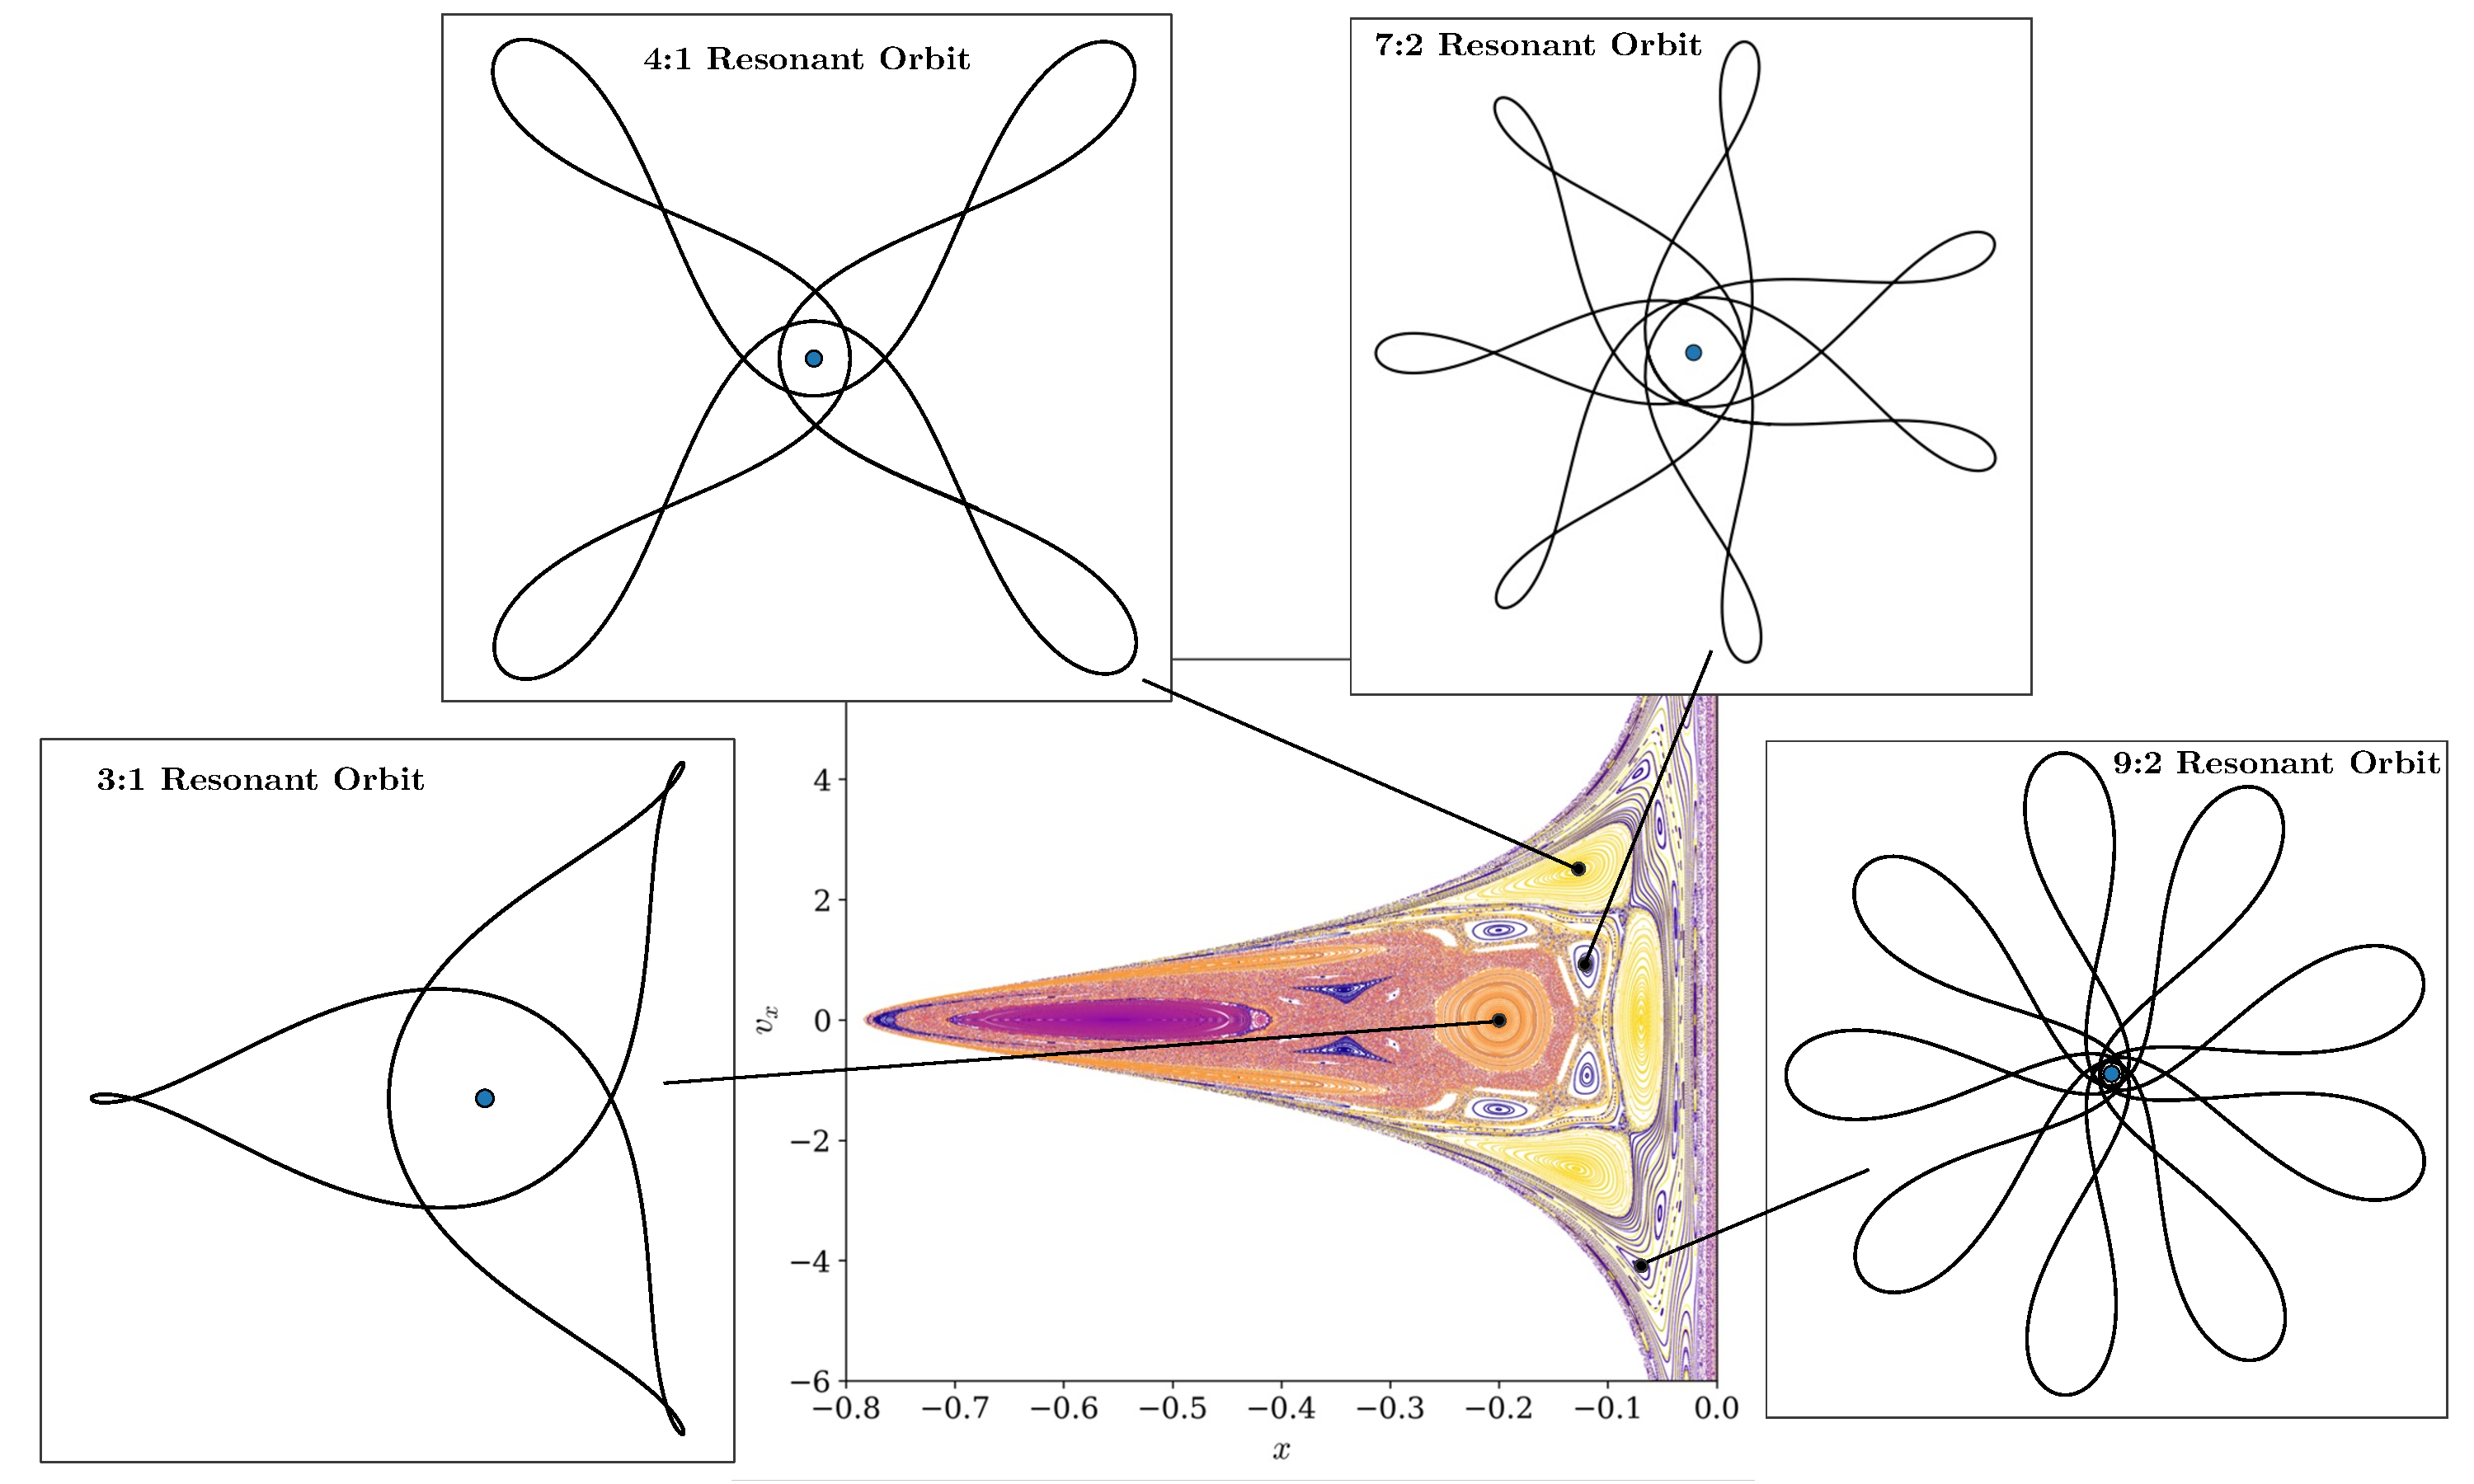
\includegraphics[width=0.7\linewidth]{images/Chaotic_sea_figure.pdf}
        \caption{Depiction of several stable points in the $C=3.2$ diagram corresponding to low ratio $p:q$ resonant orbits.}
        \label{fig: Jannik's nice poincare pq diagram}
    \end{figure}